\documentclass[conference]{IEEEtran}
\usepackage{graphicx}
\usepackage{caption}
\usepackage{subcaption}
\usepackage{hyperref}
\usepackage{tikz}
\usepackage{float}
\usepackage{amsmath}
\usepackage{algorithm}
\usepackage{algpseudocode}

\begin{document}

\title{SolidAttention Trade-off Study \& Flexible Data Placement (FDP) Based Optimization for LLM Inference}

\author{\IEEEauthorblockN{Guy Pinsker}
\IEEEauthorblockA{\textit{Technion - Israel Institute of Technology} \\
Information in Storage Systems, Spring 2026}}

\maketitle

\begin{abstract}
    Memory constraints of modern PCs/laptops pose a significant bottleneck for serving Large Language Models (LLMs) inference locally, mainly due to the linear growth of the Key-Value (KV) cache. The \textit{SolidAttention} framework offers a clever workaround by offloading the KV cache onto SSD storage, exploiting dynamic attention sparsity to load only relevant cache blocks (each containing multiple K-V pairs). However, this introduces a fundamental conflict between fine-grained sparse attention and the coarse-grained sequential access patterns optimal for SSDs. 

    This report describes the simulation and evaluation of the model's accuracy vs. inference throughput (tokens/sec) trade-off in \textit{SolidAttention} across various block sizes. Furthermore, it describes and presents simulated results of a proposed hardware-level optimization: Using NVMe Flexible Data Placement (FDP) to segregate cache data, reducing Garbage Collection (GC) latency spikes and increasing bandwidth via cross-channel striping. Simulation results show that combining \textit{SolidAttention} with FDP can effectively pushes the Pareto frontier of SSD-based inference forward.
\end{abstract}

\vspace{0.5cm}

\section{Introduction}
    
    \subsection{Background and the Memory Wall}
        Large Language Models (LLMs) have been widely adopted in recent years, showcasing impressive capabilities in reasoning, summarization, and coding. However, bringing these models to local edge devices, such as PCs/laptops with limited memory resources, remains a challenge.

        To understand the core of the problem, one must look at the Transformer attention mechanism. The self-attention operation computes a weighted sum of past token representations, mapping an input query to keys and values. Mathematically, this is expressed as $S = \text{softmax}(QK^T / \sqrt{H})V$, where $Q$ is the query vector of the current token, and $K$ and $V$ are the key and value matrices of all preceding tokens.

        Transformer-based LLM inference (e.g. Llama or Qwen models) consists of two phases: a prefill phase where the input prompt is processed in parallel, and an autoregressive decode phase where tokens are generated sequentially, one by one. To prevent redundant computation of the $K$ and $V$ matrices from scratch for every new token during the decode phase, inference engines retain the Key (K) and Value (V) tensors of all past tokens in memory. These tensors are collectively known as the KV cache.

        As the context length of LLMs extends to 128k tokens and beyond, the KV cache grows linearly (for each new token generated, it's corresponding new Key and Value vectors must also be stored in the cache, for future tokens generation). For an 8-billion parameter model, storing a 128k-token KV cache in 16-bit precision requires over 16 GB of memory—surpassing the size of the model weights themselves, as illustrated in Figure \ref{fig:solid_kv_size}. This memory overhead exceeds the 8 to 16 GB DRAM/VRAM capacities commonly found in consumer PCs, exposing a severe "memory wall". 

        While techniques such as INT8/INT4 quantization can compress the KV cache, they are often too aggressive and lead to a severe degradation in model accuracy, especially with the rise of numerical outliers in the activation tensors. Instead, to overcome this memory wall, another approach is to offload the KV cache to slower, but larger, storage mediums, such as SSDs. Such approach is demonstrated in \textit{SolidAttention}\cite{solidattention}.

        \begin{figure}[H]
            \centering
            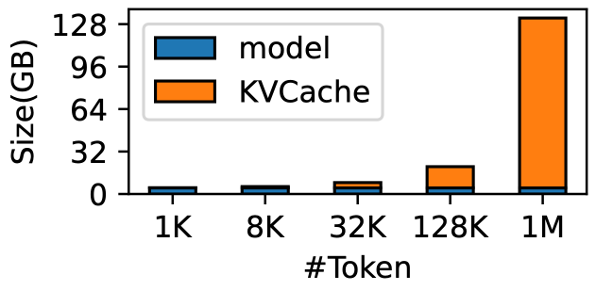
\includegraphics[width=0.9\linewidth]{figures/solid_kv_size.png}
            \caption{Memory consumption scaling (Adapted from Zheng et al.).}
            \label{fig:solid_kv_size}
        \end{figure}
    
    \subsection[SolidAttention: Low-Latency SSD-based Serving on Memory-Constrained PCs]{SolidAttention: Low-Latency SSD-based Serving on \\Memory-Constrained PCs}
        To overcome the memory wall without compromising accuracy, recent systems have explored offloading the KV cache to high-speed NVMe SSDs. \textit{SolidAttention}\cite{solidattention} is a state-of-the-art inference engine that enables SSD-based inference by co-designing sparse attention algorithms with storage management. It relies on the observation that LLM self-attention exhibits high dynamic sparsity; only a small subset of historical tokens heavily influences the generation of the current token. This means that when generating the next token, the model calculates the $QK^T$ similarity scores, but typically only a small fraction of the previous tokens return high similarity values. Therefore, instead of loading the entire KV cache from the SSD at every step, it is possible to retrieve only the necessary past tokens to compute the next token.

        \begin{figure}[H]
            \centering
            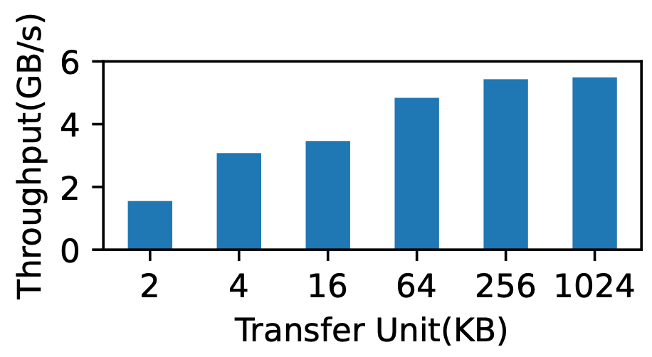
\includegraphics[width=0.9\linewidth]{figures/solid_throughput.png}
            \caption{SSD read throughput (Adapted from Zheng et al.).}
            \label{fig:solid_throughput}
        \end{figure}

        However, as learned during the course and as verified by the authors (and seen in Figure \ref{fig:solid_throughput}), SSDs reach their peak performance only when reading large, sequential chunks of data. Reading small, scattered chunks (such as the dynamically selected sparse tokens) results in poor bandwidth utilization due to the internal architecture of flash memory, which relies on channel-level parallelism to achieve high speeds. This disparity between the fine-grained data needs of the LLM and the coarse-grained throughput requirements of the SSD sets the stage for the \textit{SolidAttention}\cite{solidattention} architecture, shown in Figure \ref{fig:solid_architecture}.

        \begin{figure}[H]
            \centering
            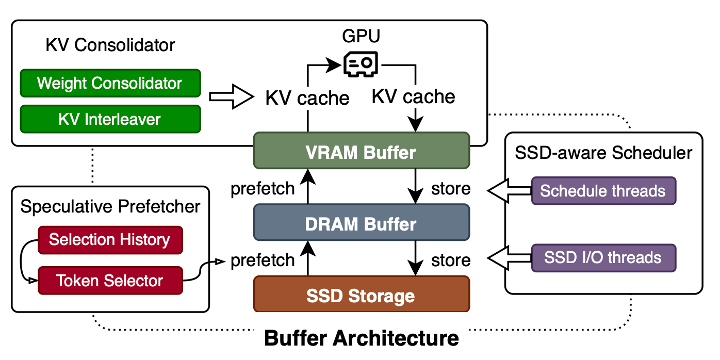
\includegraphics[width=0.9\linewidth]{figures/solid_architecture.png}
            \caption{Architecture overview of SolidAttention (Adapted from Zheng et al.). The framework coordinates a KV Consolidator, a Speculative Prefetcher, and an SSD-aware Scheduler to hide I/O latency (Adapted from Zheng et al.).}
            \label{fig:solid_architecture}
        \end{figure}

        To bridge this gap, \textit{SolidAttention}\cite{solidattention} introduces a \textbf{KV Consolidator} (Figure \ref{fig:solid_kv_consolidator}). In typical frameworks, Key and Value tensors are stored separately in memory. \textit{SolidAttention}\cite{solidattention} physically interleaves them token-by-token. By doing this, whenever the model needs a token, the system can fetch its Key and Value simultaneously in a single, contiguous read operation. This doubles the transfer unit size and halves the total number of I/O operations, maximizing SSD bandwidth utilization.

        \begin{figure}[H]
            \centering
            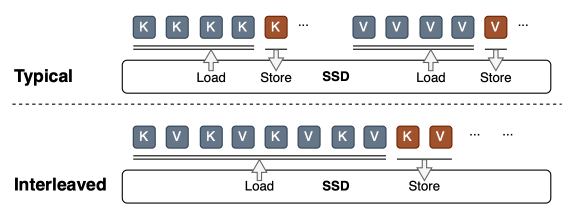
\includegraphics[width=0.9\linewidth]{figures/solid_kv_consolidator.png}
            \caption{Comparison of memory layouts (Adapted from Zheng et al.). SolidAttention interleaves Key and Value pairs to double the transfer size, improving SSD bandwidth utilization.}
            \label{fig:solid_kv_consolidator}
        \end{figure}
        
        Furthermore, \textit{SolidAttention}\cite{solidattention} adopts the block-wise attention sparsity approach, partitioning the KV cache into coarse-grained blocks along the sequence dimension, where each block consists of several tokens. \textit{SolidAttention}\cite{solidattention} maintains three categories of blocks:

        \begin{enumerate}
            \item \textbf{Init Blocks}: The first few tokens of the prompt. Models naturally depend heavily on these initial tokens to anchor their attention distributions (a phenomenon widely known as the "attention sink").
            \item \textbf{Local Blocks}: A sliding window of the most recent tokens, which are needed to understand the immediate syntactic context.
            \item \textbf{Dynamic Selected Blocks}: Older, historically distant tokens that are dynamically chosen based on their query-key similarity scores (chosen if the model computes that their content is highly relevant to the current query token).
        \end{enumerate}
        
        To avoid stalling the GPU while waiting for the SSD to fetch the Dynamic blocks, \textit{SolidAttention}\cite{solidattention} utilizes a \textbf{Speculative Prefetcher}. Since attention sparsity exhibits strong temporal locality (the blocks chosen for the previous token generation are highly likely to be chosen for the current token generation), the prefetcher speculatively fetches the blocks that will be needed and streams them from the SSD into memory in the background. If a prediction is incorrect, the system simply issues a lightweight correction process to fetch the missing blocks, overwriting the incorrectly prefetched data in-place, without needing to reorder the cache. This is because the self-attention operation only requires each K/V pair to remain aligned, thus the physical ordering of KV pairs in the cache does not need to match their original token order. Therefore, an incorrectly prefetched block can be overwritten in-place without an additional reordering step. According to the authors, they observed approximately 81\% similarity in block selections across consecutive iterations.

        In order to orchestrate SSD operations and GPU computations, \textit{SolidAttention}\cite{solidattention} relies on an \textbf{SSD-aware Scheduler}. The scheduler receives an execution plan from the inference framework and coordinates GPU computations with concurrent SSD I/O. Breaking the attention computation into microtasks allows it to pipeline fine-grained operations and I/O based on data dependencies (using a DAG representation).

        While highly effective, the performance of \textit{SolidAttention}\cite{solidattention} is still susceptible to the performance characteristics of the SSD and its internal operations, mainly the SSD's garbage collection (GC) process. Since the LLM's KV cache is massive and constantly updated, it frequently triggers GC, which can cause unpredictable latency spikes that stall the GPU. This is particularly problematic for scenarios requiring low latency, such as LLM interactions on PCs/laptops.
    
    \subsection{Flexible Data Placement (FDP)}
        As learned during the course, data in SSDs is written in page granularity, while the process of erasing is performed in block granularity (a block typically contains many pages). Moreover, pages cannot be overwritten directly - in order to overwrite a page, it must first be erased. The SSD controller constantly writes new data to fresh pages (using over-provisioning) and updates a Logical-to-Physical (L2P) mapping table. The old, obsolete pages are marked as invalid. When free pages become scarce, the SSD must perform a background process called \textbf{Garbage Collection (GC)}: it reads the remaining valid pages from a partially empty block, copies them to a new block, and then erases the entire old block. This process induces extra, unnecessary write traffic, known as Write Amplification (WA).
        
        During LLM inference, specifically throughout the autoregressive decode phase, the system continuously appends newly generated Key-Value (KV) pairs to the SSD. This massive, sustained write workload rapidly depletes the SSD's free block pool, forcing aggressive, mid-session Garbage Collection. This reactive GC traffic saturates the SSD's internal channels and causes read latency spikes. Consequently, when the inference engine's speculative prefetcher attempts to asynchronously load KV blocks, these GC-induced stalls disrupt the tight computation-I/O overlap, degrading token generation throughput.
        
        NVMe Flexible Data Placement (FDP) (TP4146) is a new storage standard that gives the host computer direct control over where data is physically placed on the SSD. Instead of letting the SSD controller mix all incoming data into the same physical blocks, FDP allows the host to tag write commands with specific identifiers called Reclaim Unit Handles (RUHs). The SSD maps these tags to isolated physical areas called Reclaim Units (RUs) within larger Endurance Groups, ensuring that data streams with similar lifespans are grouped together at the hardware level.

        An example of FDP process is shown in Figure \ref{fig:fdp_example}.
        \begin{figure}[H]
            \centering
            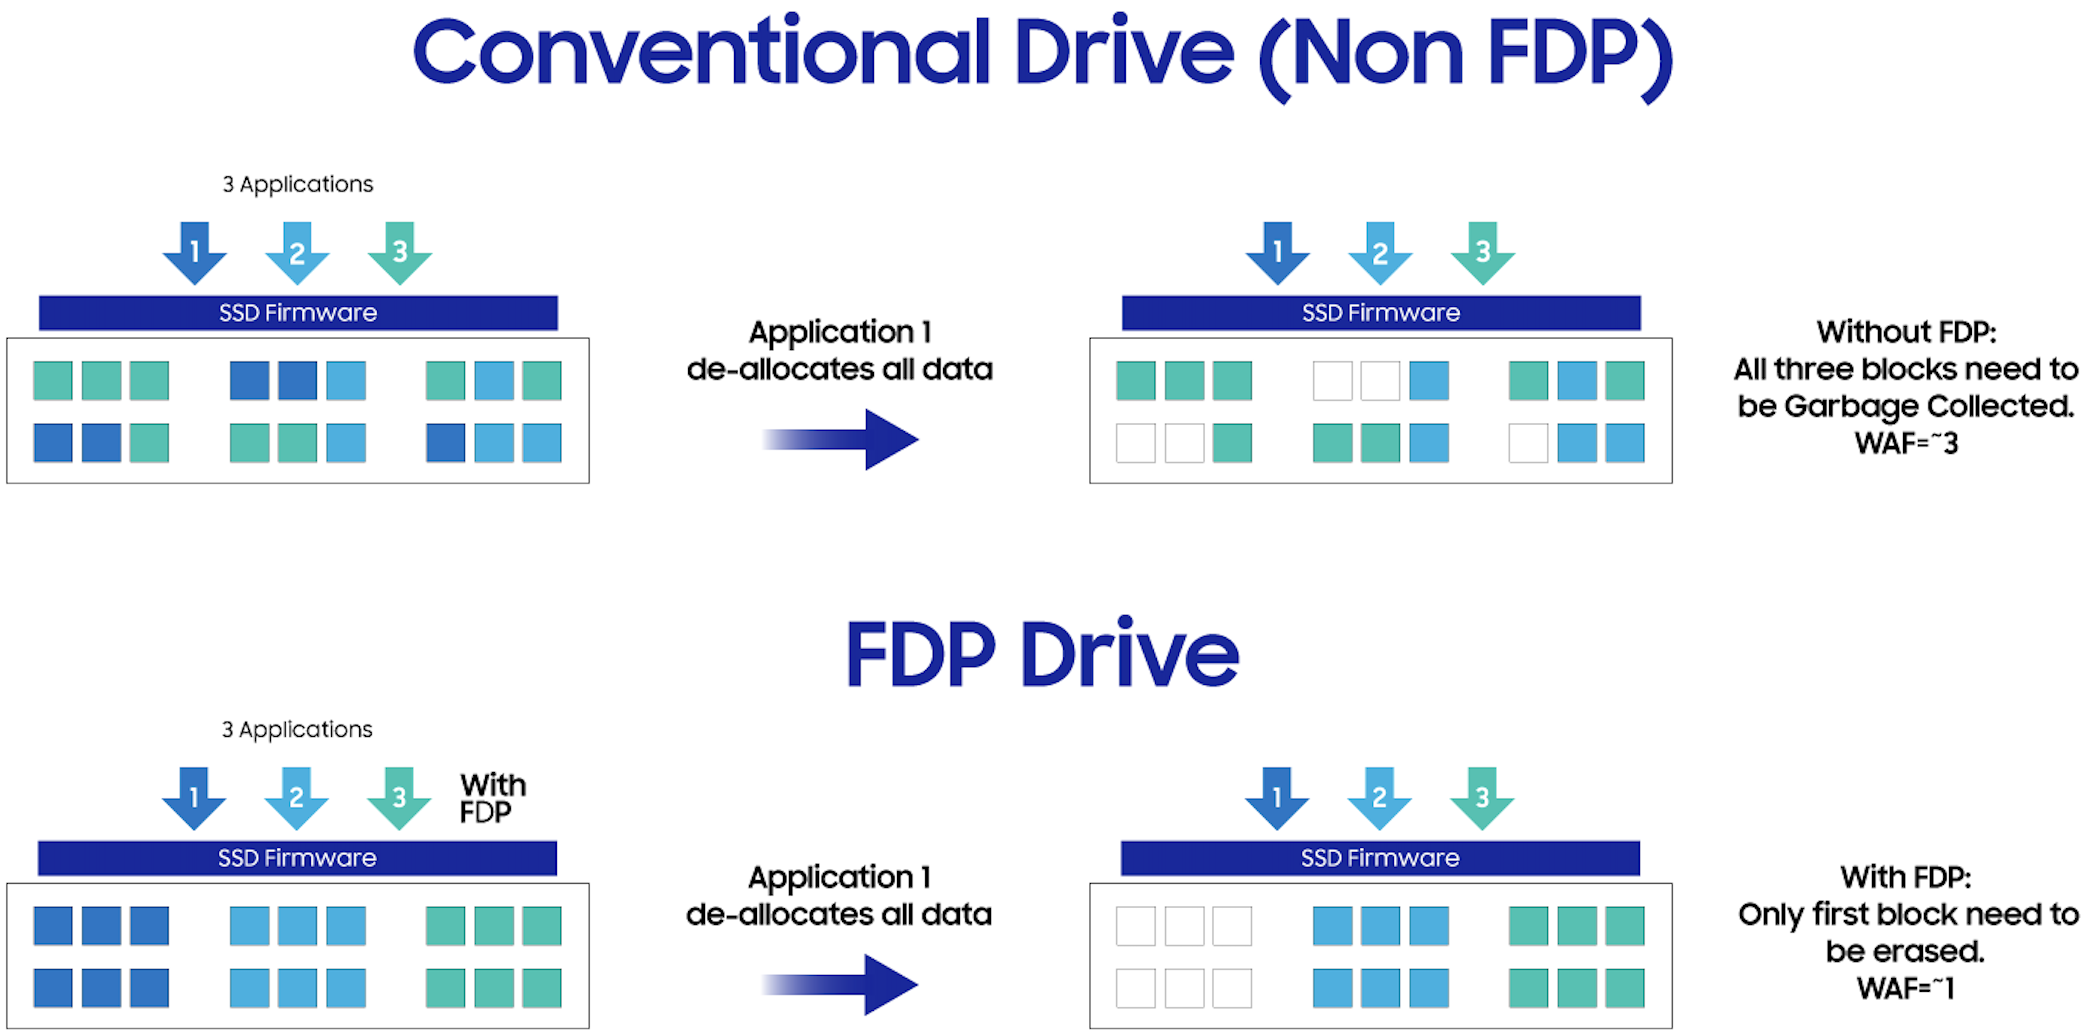
\includegraphics[width=0.9\linewidth]{figures/fdp_example.png}
            \caption{An example of FDP in action (Adapted from Samsung Semiconductor\cite{fdp_overview}).}
            \label{fig:fdp_example}
        \end{figure}

        For the SolidAttention architecture, FDP provides a powerful hardware-level isolation mechanism. It allows the host to physically segregate the application-specific LLM data (the entire KV cache for a given inference session) from the general background data of the SSD. Because the gigabytes of KV cache are quarantined in their own dedicated RUs, under an idealized FDP placement in which session data is grouped by lifetime, the inference workload can avoid relocation of still-valid KV pages during the active session. Under this ideal scenario, the inference workload induces absolutely zero Garbage Collection on its own data during the session. The blocks fill sequentially with entirely valid data, preventing the drive from entering reactive GC. When the inference request completes, the host issues an NVMe Deallocate (TRIM) command targeting those specific RUs, instantly dropping them to zero percent valid data so the SSD can erase the blocks without relocating a single page. Furthermore, by striping these session-specific RUHs across multiple physical NAND channels, FDP may enable more predictable and efficient placement of the session's data across the SSD's available parallel resources.

        While the authors of SolidAttention mention that the frequent KV cache write cause write amplifications, and that they found their performance overhead negligible compared to read operations, they did not mention the Garbage Collection process that affects the read operations as well. Thus, FDP can still be beneficial for the SolidAttention framework.

\section{The Project}
    \subsection{Motivation}
        From the \textit{SolidAttention}\cite{solidattention} paper, I found several key observations:
        \begin{enumerate}
            \item SSD performance improves with larger transfers.
            \item Larger blocks reduce attention-selection quality. 
        \end{enumerate}
        Therefore, there is a storage/ML Pareto frontier. Changing the storage system could move that frontier.
        Hence the primary objective of this project was to empirically evaluate the accuracy vs. throughput trade-off of the \textit{SolidAttention}\cite{solidattention} framework and construct a robust simulation environment to validate the hypothesis that FDP could improve the storage side of the tradeoff.
        
        \subsection{Methodology}
            The project workflow is structured into three interconnected phases:

        \subsubsection*{\textbf{Phase 1: Storage Profiling}}
            To ensure my simulations were grounded in physical reality, I first measured how fast my actual laptop SSD could serve random read requests. I utilized the \texttt{fio} (Flexible I/O Tester) benchmarking tool, configuring it to bypass the operating system cache (\texttt{direct=1}) to simulate true raw hardware performance. I tested the SSD's read throughput across a spectrum of chunk sizes (e.g., 2KB, 4KB, 8KB, 16KB), in a random read workload of a 10 GB file.

        \subsubsection*{\textbf{Phase 2: Model Accuracy Profiling}}
            While larger block sizes yield higher SSD throughput (as loading and writing data occurs at coarser granularity), they negatively impact the precision of the dynamic attention sparsity algorithm. The system chooses which blocks are needed by looking at the representative vector of each block. If the block size is too large, attention sparsity will cause tokens that are semantically important to be surrounded by unrelated tokens that act as noise, within the same block. Therefore, the representative vector information of the relevant token will be diluted, thus the block may not achieve a high enough attention score, and will not be selected. This can cause the system to retrieve irrelevant tokens at the expense of relevant ones, corrupting the context and degrading the model's generative accuracy.

            To quantify this, I utilized a "Needle-In-A-Haystack" testing framework. This test, prevalent in the field of accuracy evaluations of LLMs, involves embedding a specific piece of information (the "needle") deep within a massive corpus of background text (the "haystack") and prompting the model to retrieve it. To ensure the test was robust and representative of dense knowledge retrieval, I built the haystacks using raw text extracted directly from the Wikipedia pages for \textit{"The United States"} and \textit{"World War II"}. The "needle" was the phrase: \textit{"The secret code word to access the vault is 'PINEAPPLE'."} It was retrieved by prompting the model with the phrase: \textit{"Question: What is the secret code word to access the vault? Answer strictly with just the single word.\textbackslash{}nAnswer:"} and allowing it to generate 5 new tokens. If the word \textit{"PINEAPPLE"} (case-insensitive) was detected in the generated text, the test was considered successful.

            Crucially, I carefully planted the needle far enough back (but not too far) in the text so that it would fall outside of the "Init" blocks (the start of the text) and the "Local" blocks (the very end of the text). This forced the model to rely entirely on the "Dynamically Selected Blocks" mechanism to retrieve the answer. I ran this test on three leading open-source models (Llama-3.1-8B, Llama-3.2-3B, and Qwen-2.5-7B, also used in the original paper), progressively varying the algorithmic block size each time to see how often the model failed to find the needle. This failure frequency formed the "miss rate" for my subsequent analyses.

        \subsubsection*{\textbf{Phase 3: Trade-off Simulation}}
            In the final phase, I wrote a custom Python latency simulator to model the entire end-to-end inference system. The simulator ingested the physical hardware speeds established in Phase 1 and merged them with the algorithmic accuracy limits discovered in Phase 2. It estimated the total wall-clock time required to generate tokens, allowing to compute the actual tokens per second throughput.

            The simulator factors in various parameters:
            \begin{itemize}
                \item {\textbf{Number of tokens to generate} An output sequence of 1000 tokens is large enough to make sure the random events (garbage collection, incorrectly prefetched blocks) will occur in significant amount.}
                \item {\textbf{Context Budget} Similar to SolidAttention, the number of tokens found in the VRAM/DRAM at a given time is no larger than 1000.}
                \item {\textbf{Number of tokens for Selected Blocks:} How many "Top-K" blocks to select. Similar to SolidAttention, this was set to 1/2 the context budget (500 tokens)}
                \item {\textbf{Size per token per layer (using FP16 K+V)} Depends on the model - 4KB for Llama, 2KB for Qwen)}
                \item {\textbf{Number of layers in the model} 32 for Llama, 28 for Qwen}
                \item {\textbf{Miss rate for speculative prefetcher} Used value of 19\%, based on SolidAttention findings. Selected blocks were randomally chosen as incorrectly prefetched based on this value.}
                \item {\textbf{Base SSD latency} Assumed a fixed value of 0.05 ms}
                \item {\textbf{Dummy compute time} Assumed 20ms for all attention and FFN computations.}
                \item {\textbf{GC spike per step probability} Assumed 5\% chance.)}
                \item {\textbf{Latency penalty of a GC spike} Assumed 50ms.}
                \item {\textbf{FDP mode} When enabled, GC probability is set to 0 and stripe multiplying is applied.}
                \item {\textbf{Multiplier for FDP striping} Assumed a multiplier of 4.}
                \item {\textbf{SSD bandwidth cap} Assumed maximum throughput of 7000 MB/s to avoid reaching unrealistic values with the striping multiplier.}
        \end{itemize}

        The Tokens/Second throughput is measured as follows:
        \begin{algorithm}
        \caption{Tokens/Second Throughput Simulation}
            \begin{algorithmic}[1]
                \Require Block size $b$ (tokens), miss rate $p_m$, SSD base latency $\ell$,
                        empirical throughput $\mathcal{T}(b)$ (MB/s), compute time $t_c$ per step,
                        GC spike probability $p_{gc}$, GC penalty $t_{gc}$, token size $\sigma$ (bytes/token/layer),
                        number of layers $L$, generation steps $N$, budget $B$ (tokens)
                \State $k \leftarrow \max\!\left(1,\, \left\lfloor B / b \right\rfloor\right)$
                \Comment{Top-$k$ blocks fetched per step}
                \State $s_b \leftarrow (b \cdot \sigma)\,/\,(1024^2)$
                \Comment{Block size in MB}
                \State $T_{\text{stall}} \leftarrow 0$,\quad $T_{\text{compute}} \leftarrow 0$
                \For{$i = 1$ \textbf{to} $N$}
                    \State $m \leftarrow \sum_{j=1}^{k} \mathbf{1}[\,\text{Uniform}(0,1) < p_m\,]$
                    \Comment{\# Missed blocks this step}
                    \State $t_{\text{io}} \leftarrow \left(\ell \cdot \mathbf{1}[m > 0]\right) + \frac{m \cdot s_b}{\mathcal{T}(b)} \cdot 1000$
                    \Comment{SSD access latency per layer (ms)}
                    \State $t_{\text{spike}} \leftarrow t_{gc} \cdot \mathbf{1}[\,\text{Uniform}(0,1) < p_{gc}\,]$
                    \Comment {GC penalty per step (ms)}
                    \State $T_{\text{stall}} \leftarrow T_{\text{stall}} + t_{\text{io}} \cdot L + t_{\text{spike}}$
                    \Comment {Update total stall time}
                    \State $T_{\text{compute}} \leftarrow T_{\text{compute}} + t_c$
                    \Comment {Update total compute time}
                \EndFor
                \State $T_{\text{total}} \leftarrow (T_{\text{compute}} + T_{\text{stall}}) \;/\; 1000$
                \Comment{Total wall time (s)}
                \State \Return $\text{Tokens/Second} \leftarrow N \;/\; T_{\text{total}}$
            \end{algorithmic}
        \end{algorithm}

        I ran the simulator in two distinct operational modes:
        \begin{itemize}
            \item \textbf{Baseline Block Storage}: This mode simulated a regular consumer NVMe SSD. I intentionally injected random latency penalties into the timeline to represent the severe Garbage Collection spikes and general congestion that naturally occur when an SSD is continuously battered by writes.
            \item \textbf{FDP Hardware Improvement}: This mode simulated an SSD with ideal Flexible Data Placement configuration, in which the KV-cache workload causes no relocation-induced GC during the active session (GC latency penalties are entirely removed from the mathematical model). Additionally, I applied a multiplier to the SSD's bandwidth to simulate the benefits of explicitly organizing the data across multiple flash channels via cross-channel striping. While over simplified, this approach can help convey the potential added benefit of using striping.
        \end{itemize}

        By evaluating these simulations, I generated Pareto frontier graphs to identify the optimal operating points balancing accuracy and speed for each setup.
        It is important to notice that the simulator uses a simplified additive latency model and therefore does not explicitly model the fine-grained computation/I/O overlap of the SolidAttention scheduler. The resulting throughput is therefore a first-order estimate rather than a cycle-accurate reproduction.

\section{Results}

    \subsection{Throughput vs. Accuracy Trade-off}
        My storage profiling tests aligned with the results of \textit{SolidAttention}\cite{solidattention}, and confirmed that SSD throughput depends heavily on how large the requests are. Figure \ref{fig:throughput_4kb} shows the baseline random read throughput for different block sizes, (with a 4KB token size). As block size increases, the read throughput (in MB/s) increase as well. This helps solidify the motivation of working in larger block granularity.

        \begin{figure}[H]
            \centering
            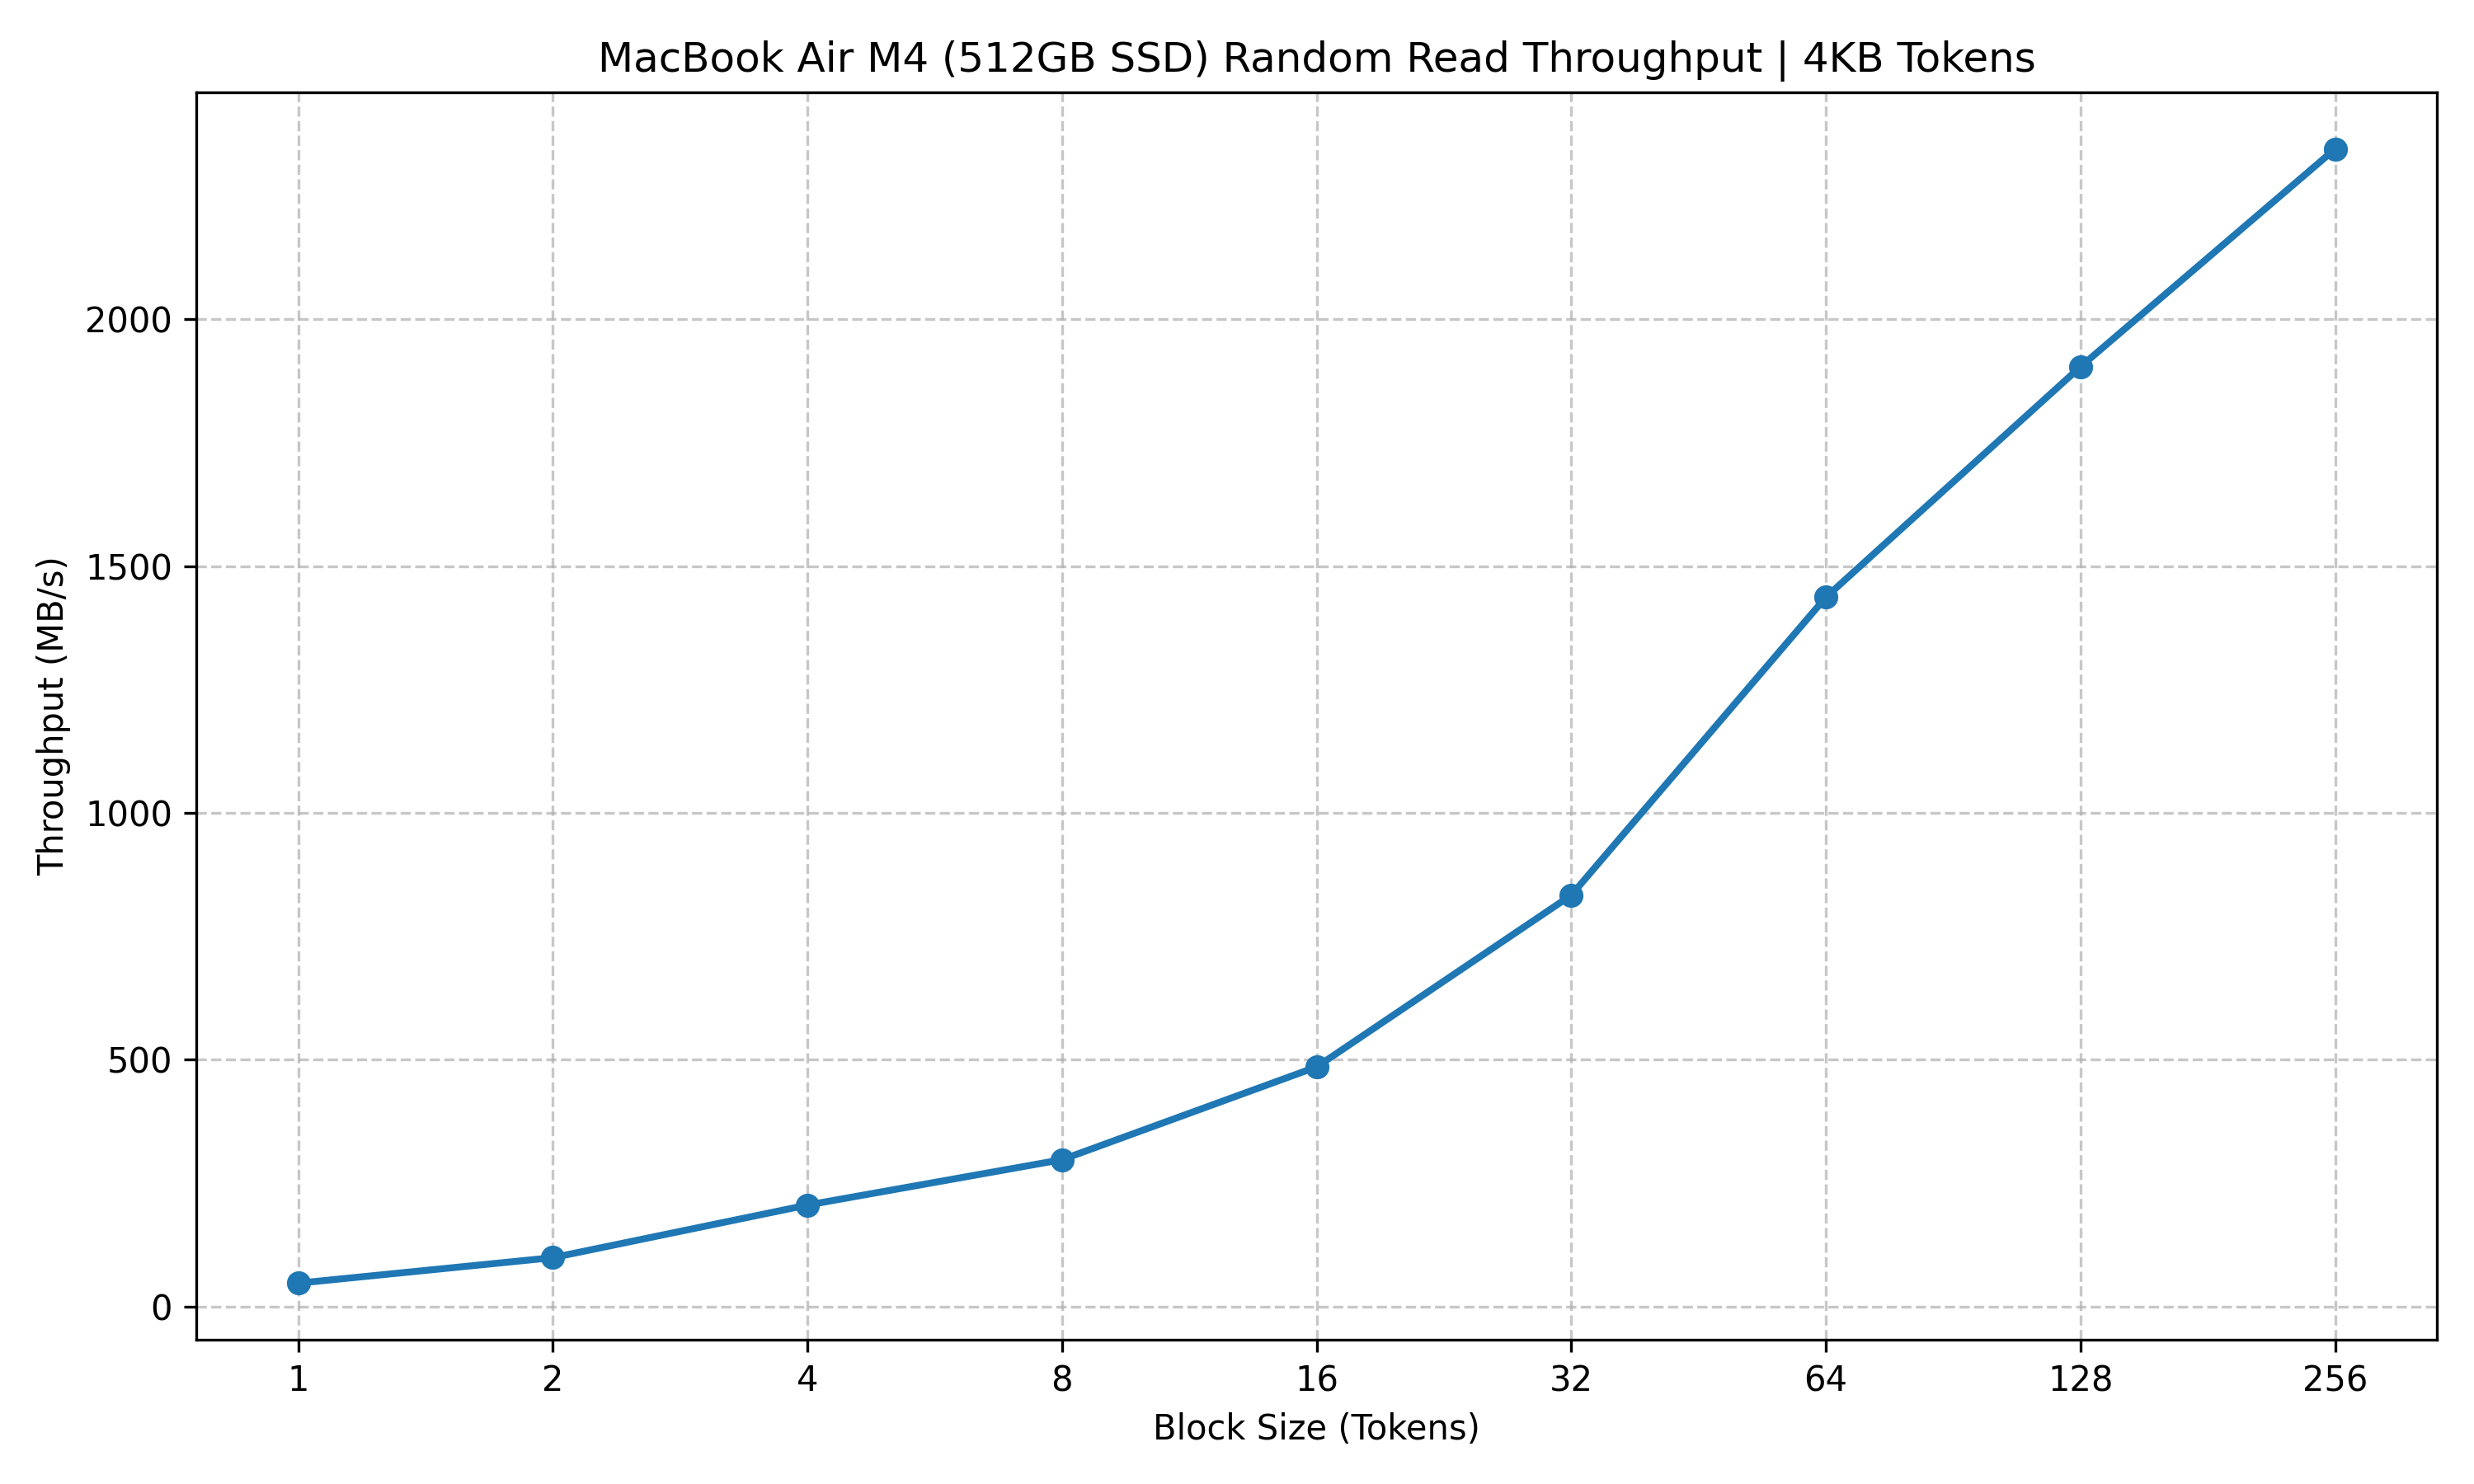
\includegraphics[width=0.8\linewidth]{../outputs/phase1/throughput_4KB_1j_1d.png}
            \caption{SSD Random Read Throughput at 4KB token size (Phase 1). Reading larger chunks is fundamentally required to maximize the SSD's physical performance.}
            \label{fig:throughput_4kb}
        \end{figure}

        However, Phase 2 laid bare the downside of this approach. 
        
        The NIAH experiment exhibits the same qualitative trend reported by \textit{SolidAttention}\cite{solidattention}: increasing block size eventually reduces retrieval quality. When looking at the actual generated answers, it was clear that the semantic importance of the needle tokens was overriden by the noise introduced by the neighboring tokens in the block. Instead of generating the correct answer, the model started generating text that was influenced by the random content of the entire block (e.g. text about the United States or WW2).
        
        Figure \ref{fig:tradeoff_llama31} shows the accuracy measured for the Llama-3.1-8B-4bit model.
        
        \begin{figure}[H]
            \centering
            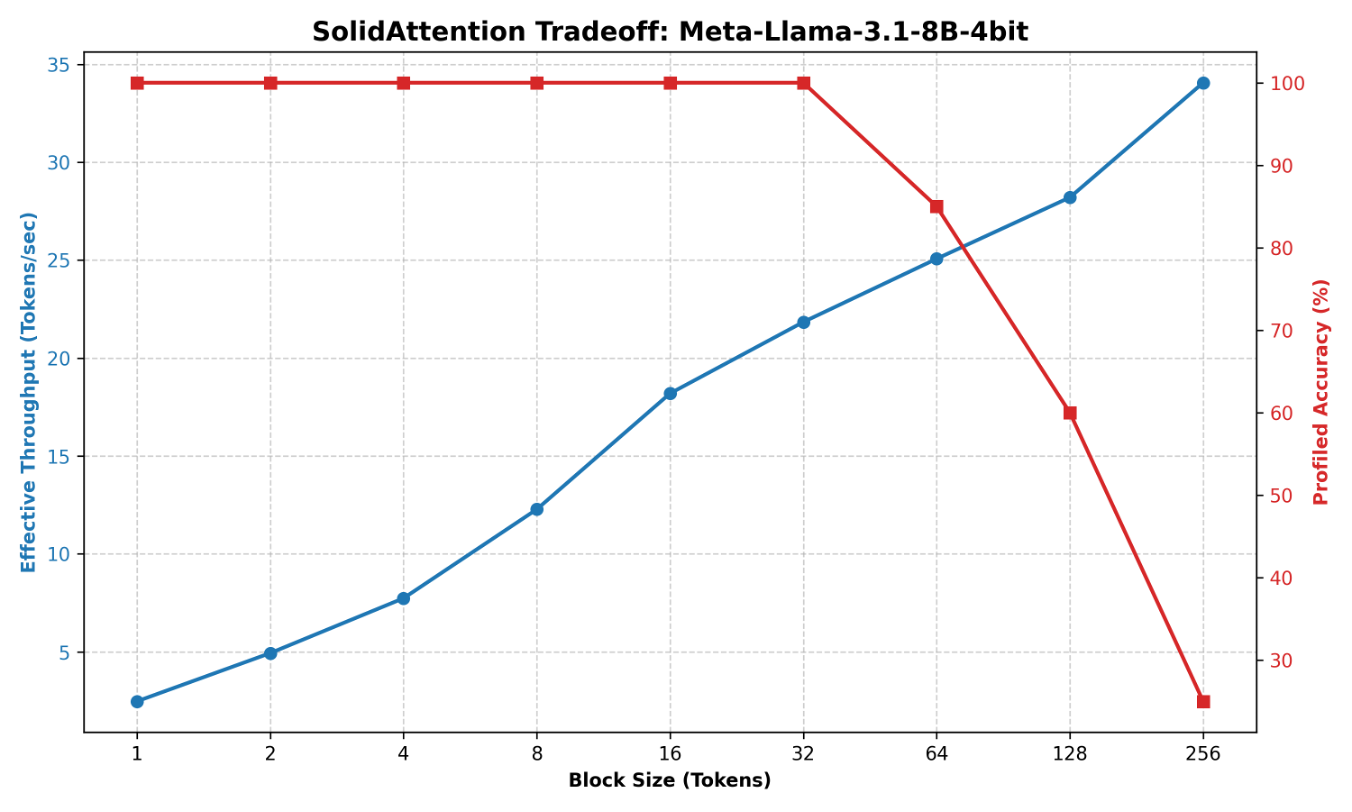
\includegraphics[width=0.8\linewidth]{../outputs/phase3/Meta-Llama-3.1-8B-4bit/solidattention_tradeoff_combined.png}
            \caption{Accuracy vs. Throughput tradeoff for Llama-3.1-8B-4bit model. This graph illustrates the direct correlation between tokens-per-second throughput and the Needle-In-A-Haystack accuracy score.}
            \label{fig:tradeoff_llama31}
        \end{figure}
        
        To better visualize the tradeoff, I generated Pareto frontiers for all the measured models, depicted in figure \ref{fig:pareto_baseline}.

        \begin{figure}[H]
            \centering
            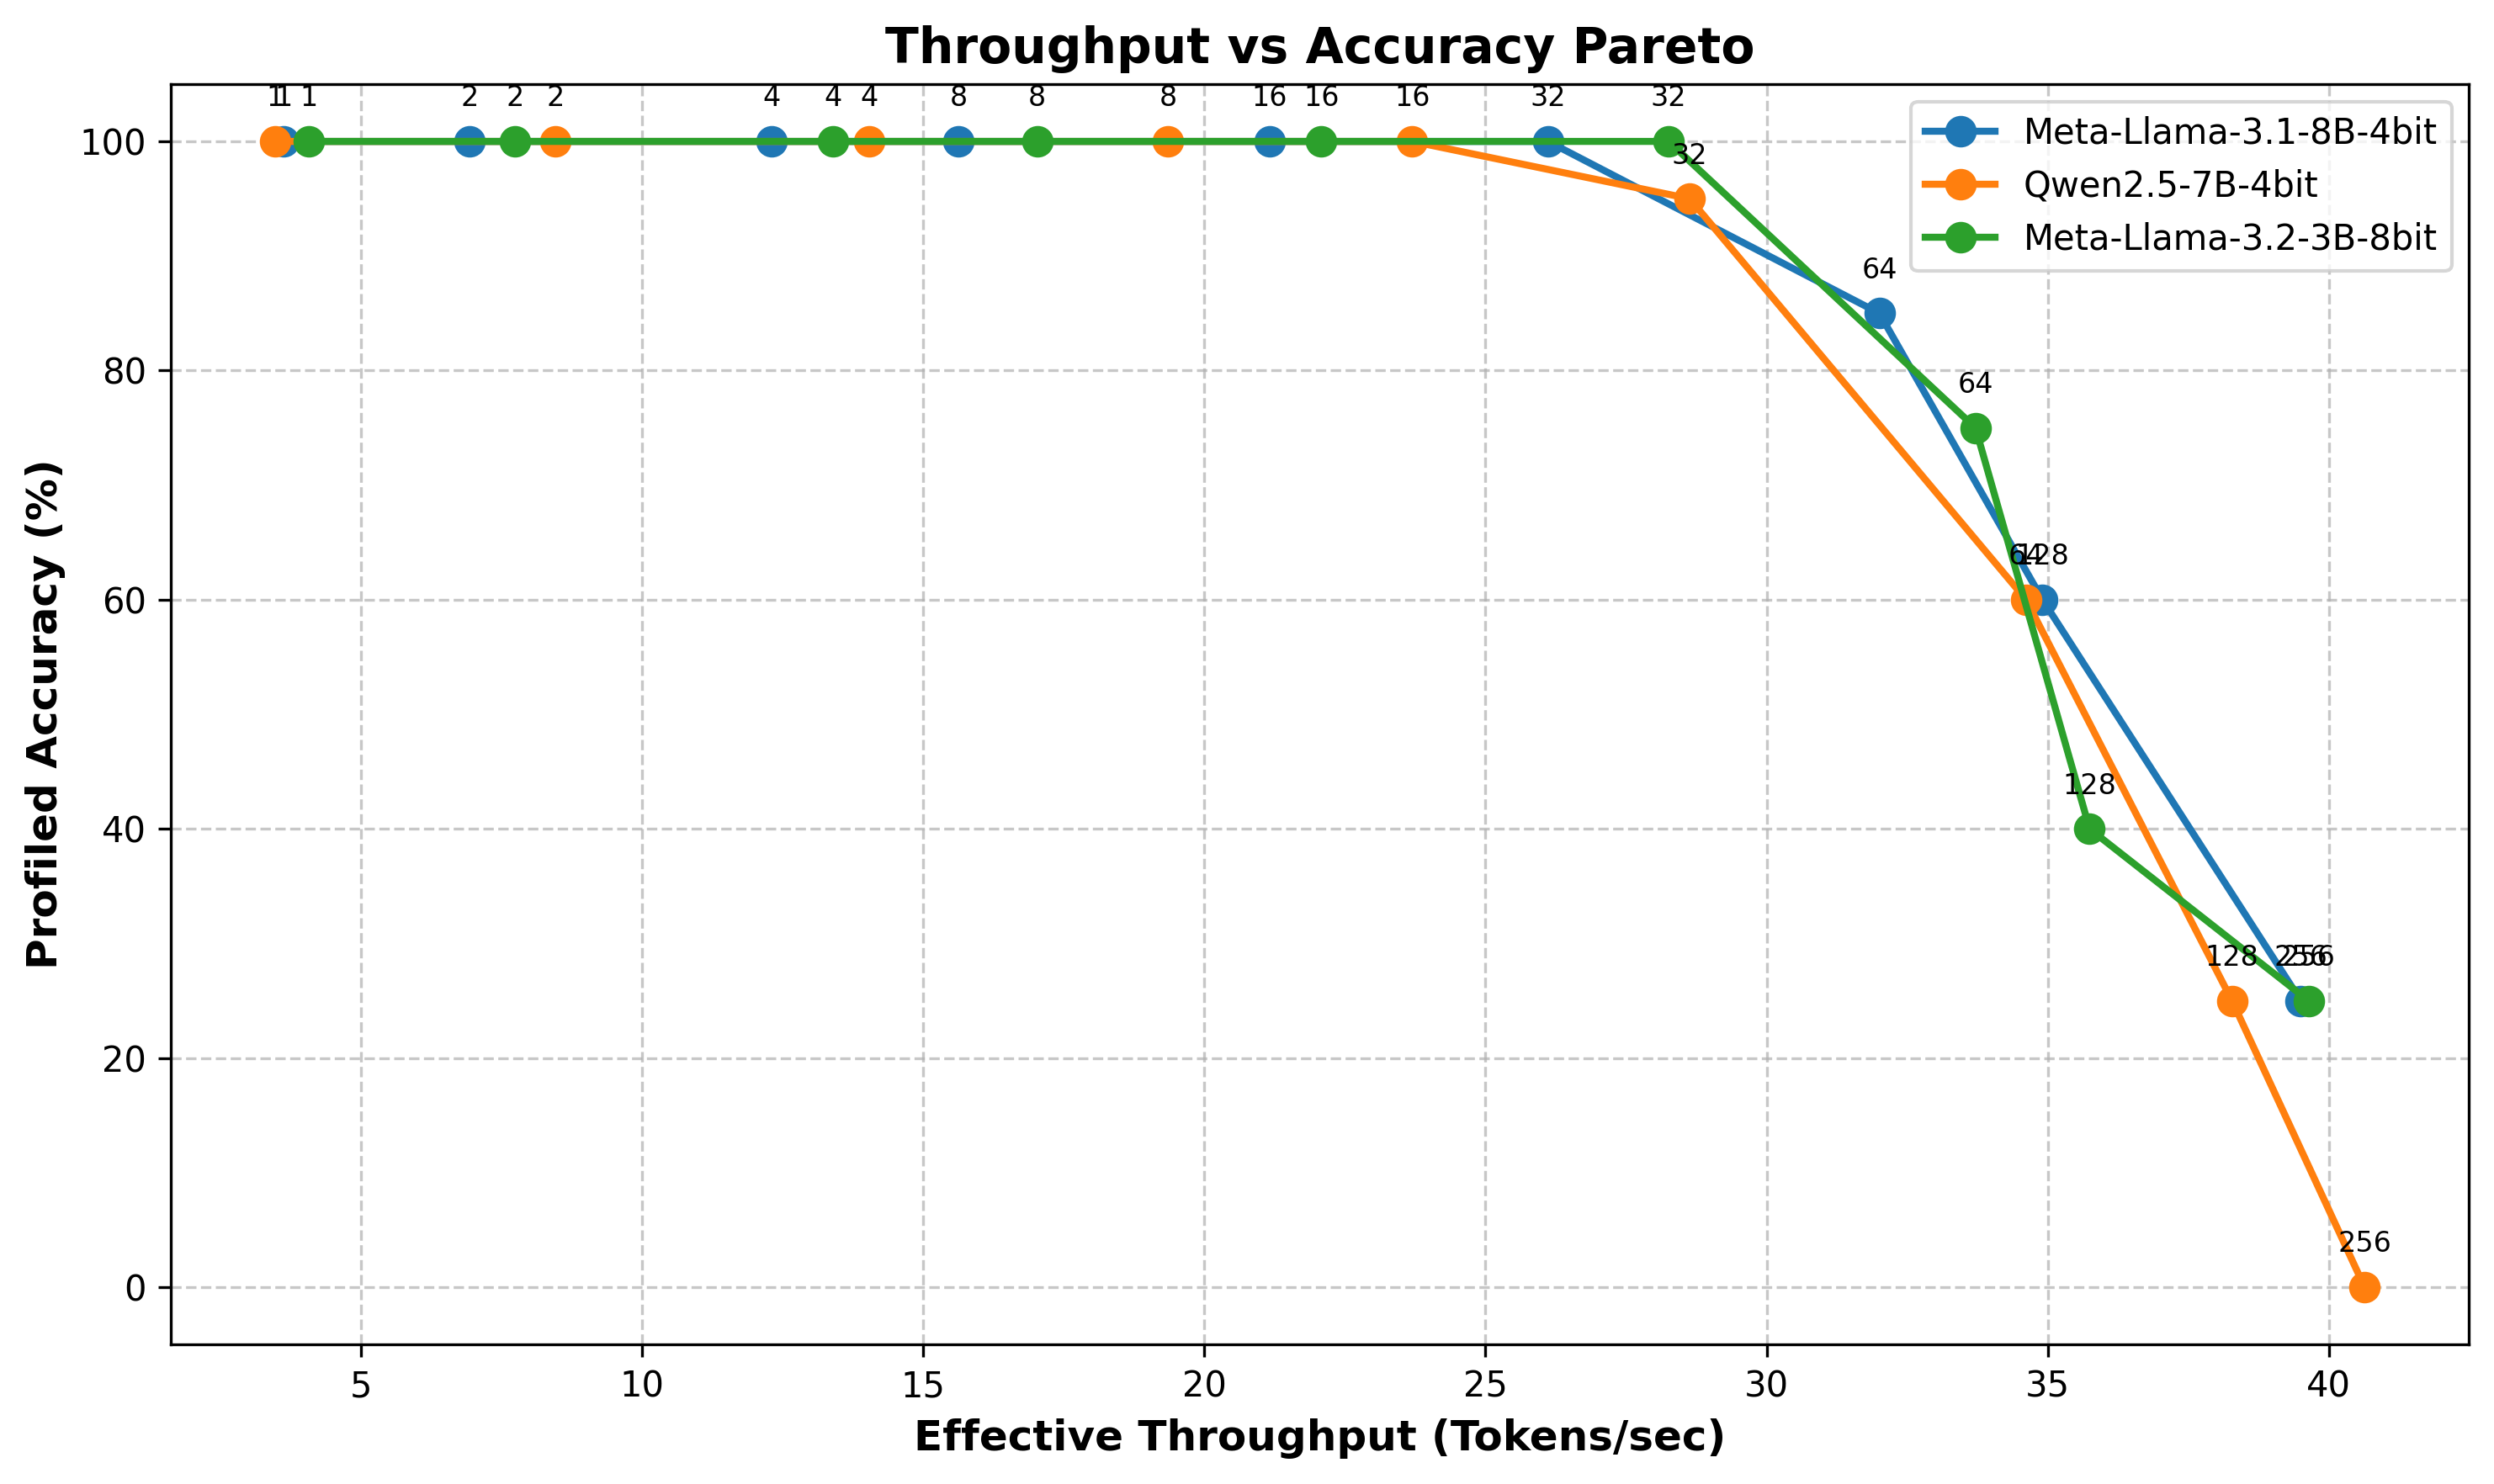
\includegraphics[width=0.8\linewidth]{../outputs/phase3/pareto_results/pareto_combined.png}
            \caption{Throughput vs. Accuracy Pareto Front for baseline models. (Phase 3)}
            \label{fig:pareto_baseline}
        \end{figure}
        
        Common to all models, both the larger 7-8 billion parameters Qwen \& Llama 3.1 and the smaller 3 billion parameters Llama 3.2, the accuracy maintains 100\% accuracy for smaller block sizes, followed by a sharp drop. However, the effective throughput (in generated tokens/second) steadily increase with block size. Overall all models exhibit similar Pareto fronts. These figures show that while increasing block size improves storage efficiency, it eventually degrades retrieval accuracy on the evaluated long-context task, especially when block size grows past 32 tokens.
        
        To further study the tradeoff, I wanted to see the infulence of the fixed miss rate, empirically established by \textit{SolidAttention}\cite{solidattention}. My motivation was to check if potentially improving the prefetching accuracy would create a significant benefit to the performance of SolidAttention, or on the other hand, see if degrading the prefetching accuracy would not signficantly impact the performance. I ran the simulation with a 30\% change to the miss rate might on the Llama-3.1-8B-4bit model. The results are shown in figure \ref{fig:pareto_miss_rate}.

        \begin{figure}[H]
            \centering
            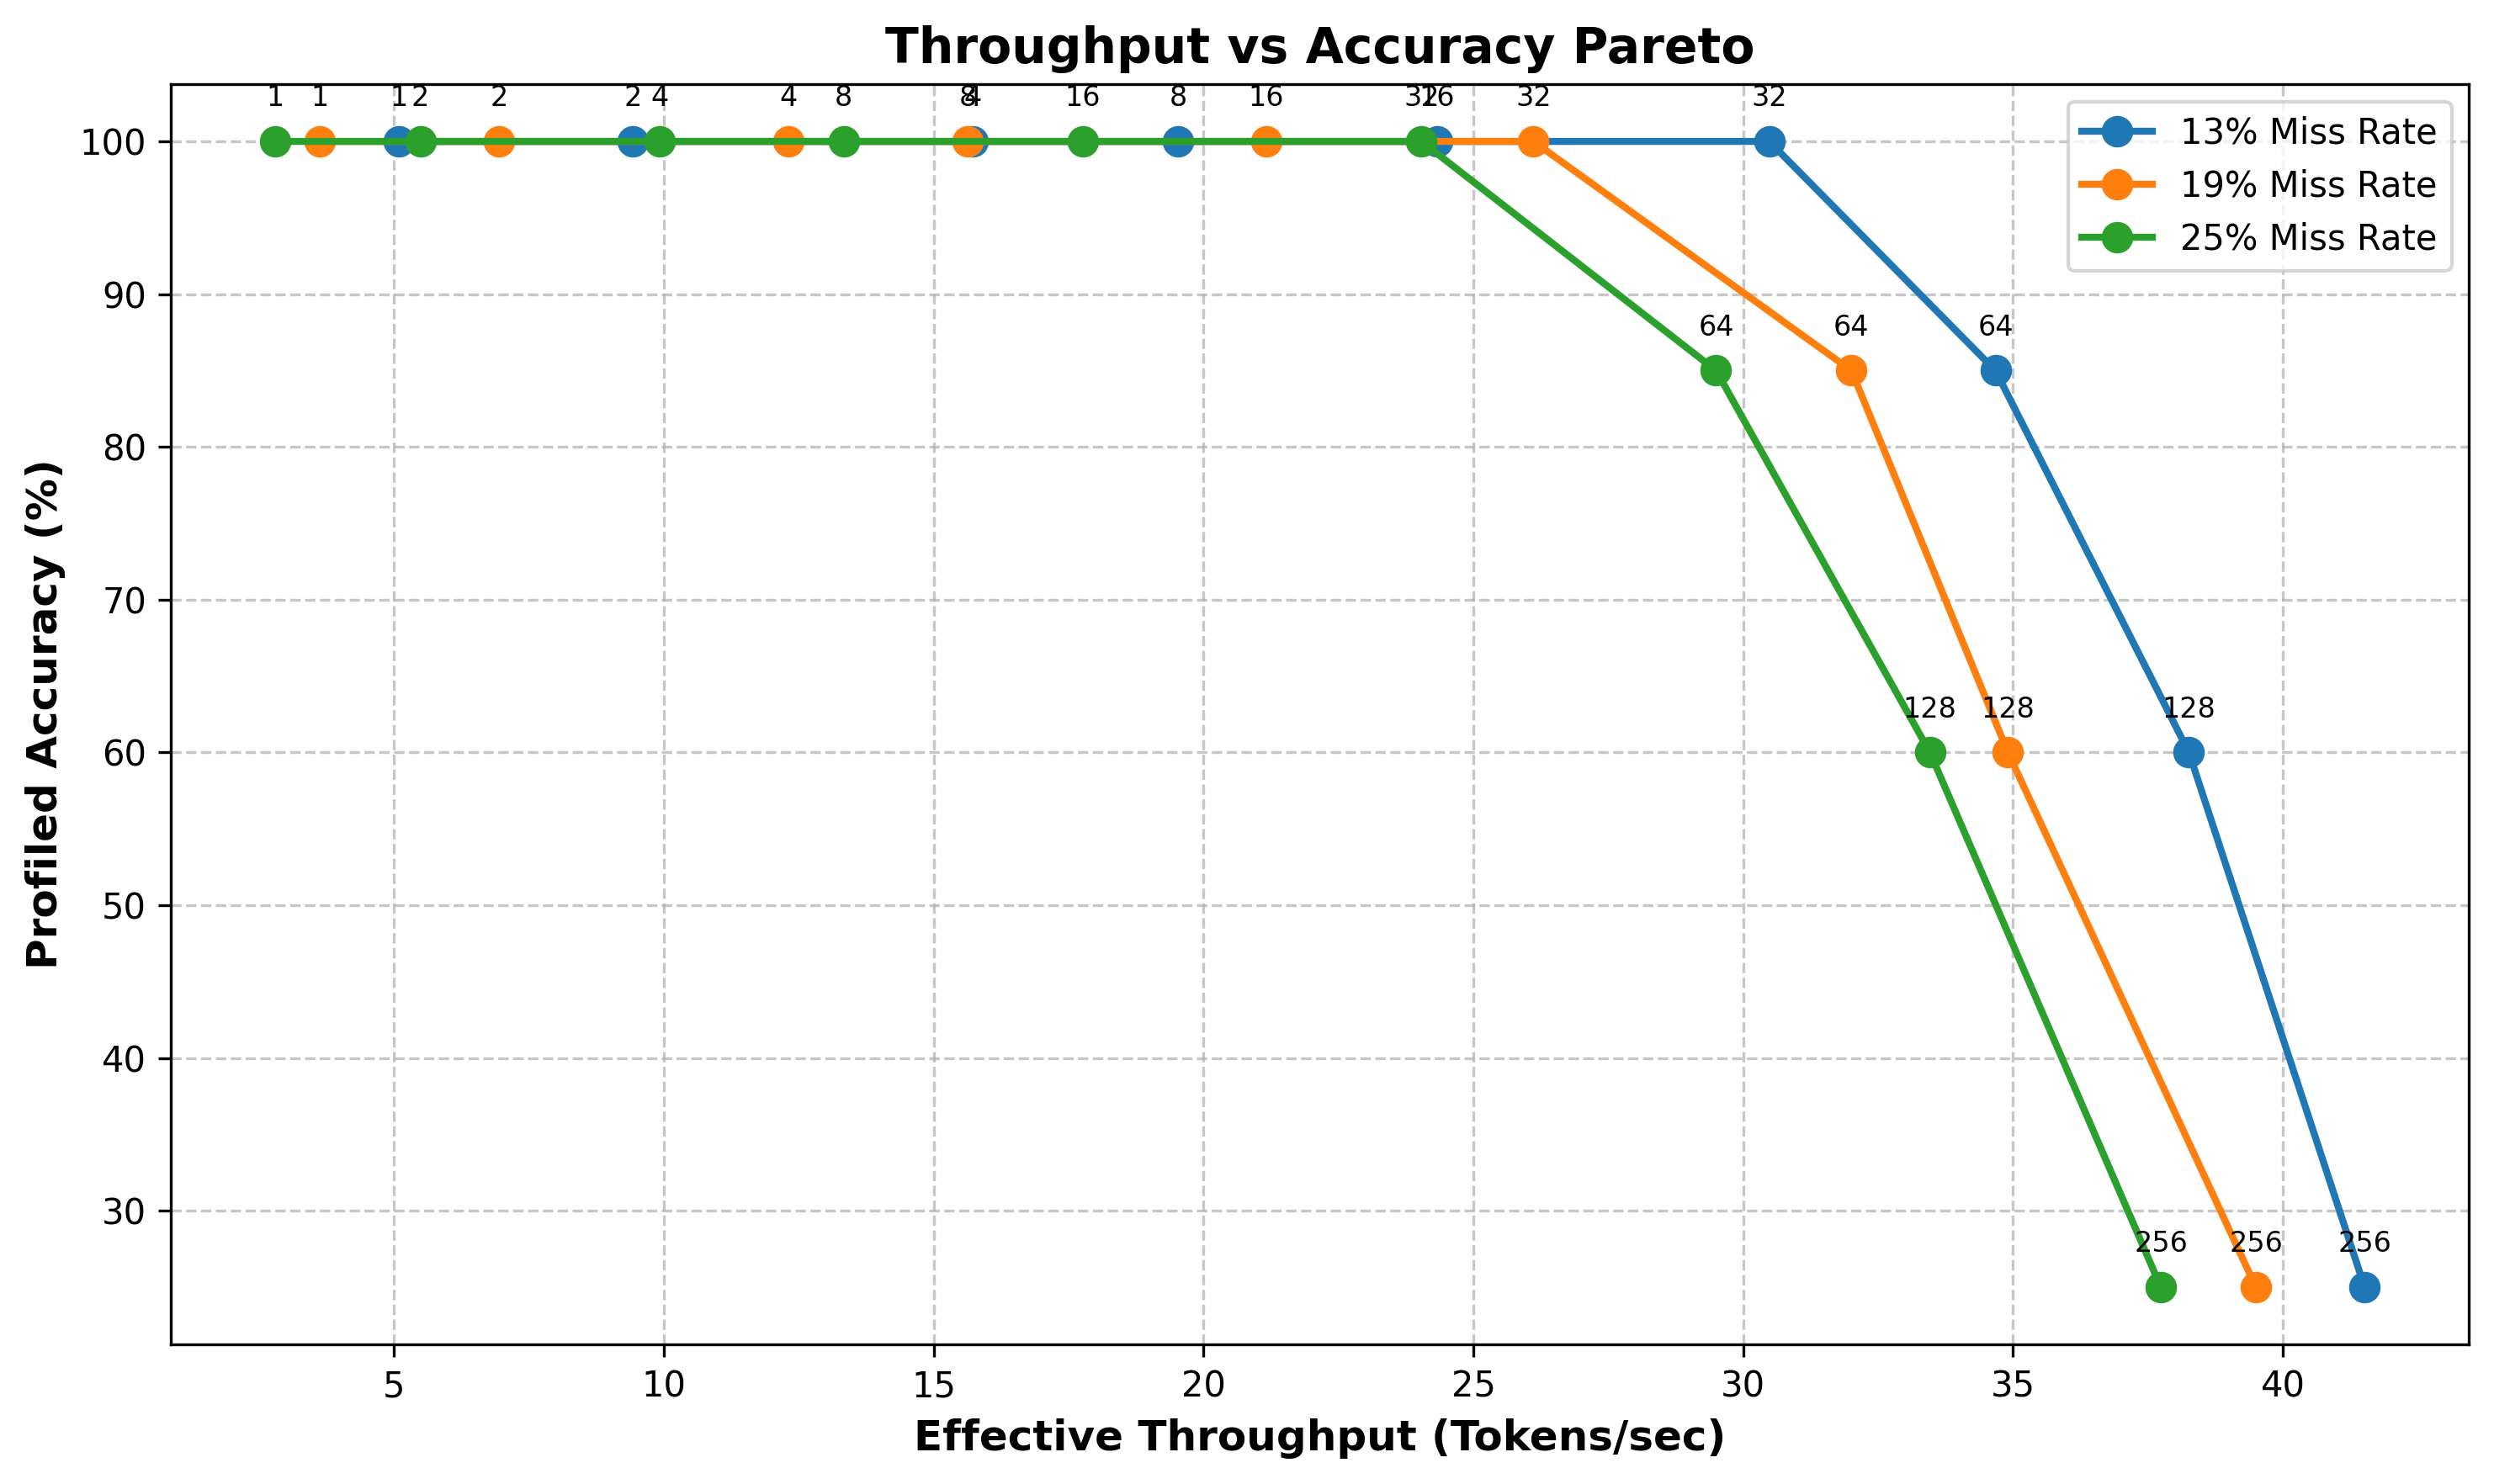
\includegraphics[width=0.8\linewidth]{../outputs/phase3/miss_rate_results/pareto_combined.png}
            \caption{Pareto Frontier for Llama-3.1-8B-4bit model, under different miss-rate values.}
            \label{fig:pareto_miss_rate}
        \end{figure}

        As can be seen in the figure, the miss rate has an asymmetrical impact on the performance of the system. Increasing the miss rate by 30\% does not significantly degrade the performance of the system, while decreasing the miss rate by 30\% generally improves the performance of the system quite significantly. This means that decreasing the miss rate might be a more effective direction for improving the performance of the system. However, since the empirically established assumption of 81\% similarity between iterations is already quite high, further improvements in prefetching accuracy might be difficult to achieve without incurring additional latency penalties (although the practical upper bound on achievable prediction accuracy remains an open question). It is worth noting that perhaps using a less accurate, but faster, prefetching algorithm could prove to be beneficial for the overall performance of the system.

    \subsection{FDP Improvement}
        Across all three models, the FDP Improvement configuration consistently pushes the simulated Pareto front significantly to the right compared to the Baseline architecture, as can be seen in figure \ref{fig:pareto_fdp_combined}. In the Baseline configuration, the "knee" of the curve (the optimal operating point where the system achieves maximum throughput without suffering severe accuracy degradation, at around a block size of 32) peaks at approximately 26-28 tokens per second. By implementing FDP with cross-channel striping, the system effectively sustains the high accuracy at substantially higher throughputs, pushing the optimal operating point to approximately 40-42 tokens per second.

        \begin{figure*}[htpb]
            \centering
            \begin{subfigure}[c]{0.32\textwidth}
                \centering
                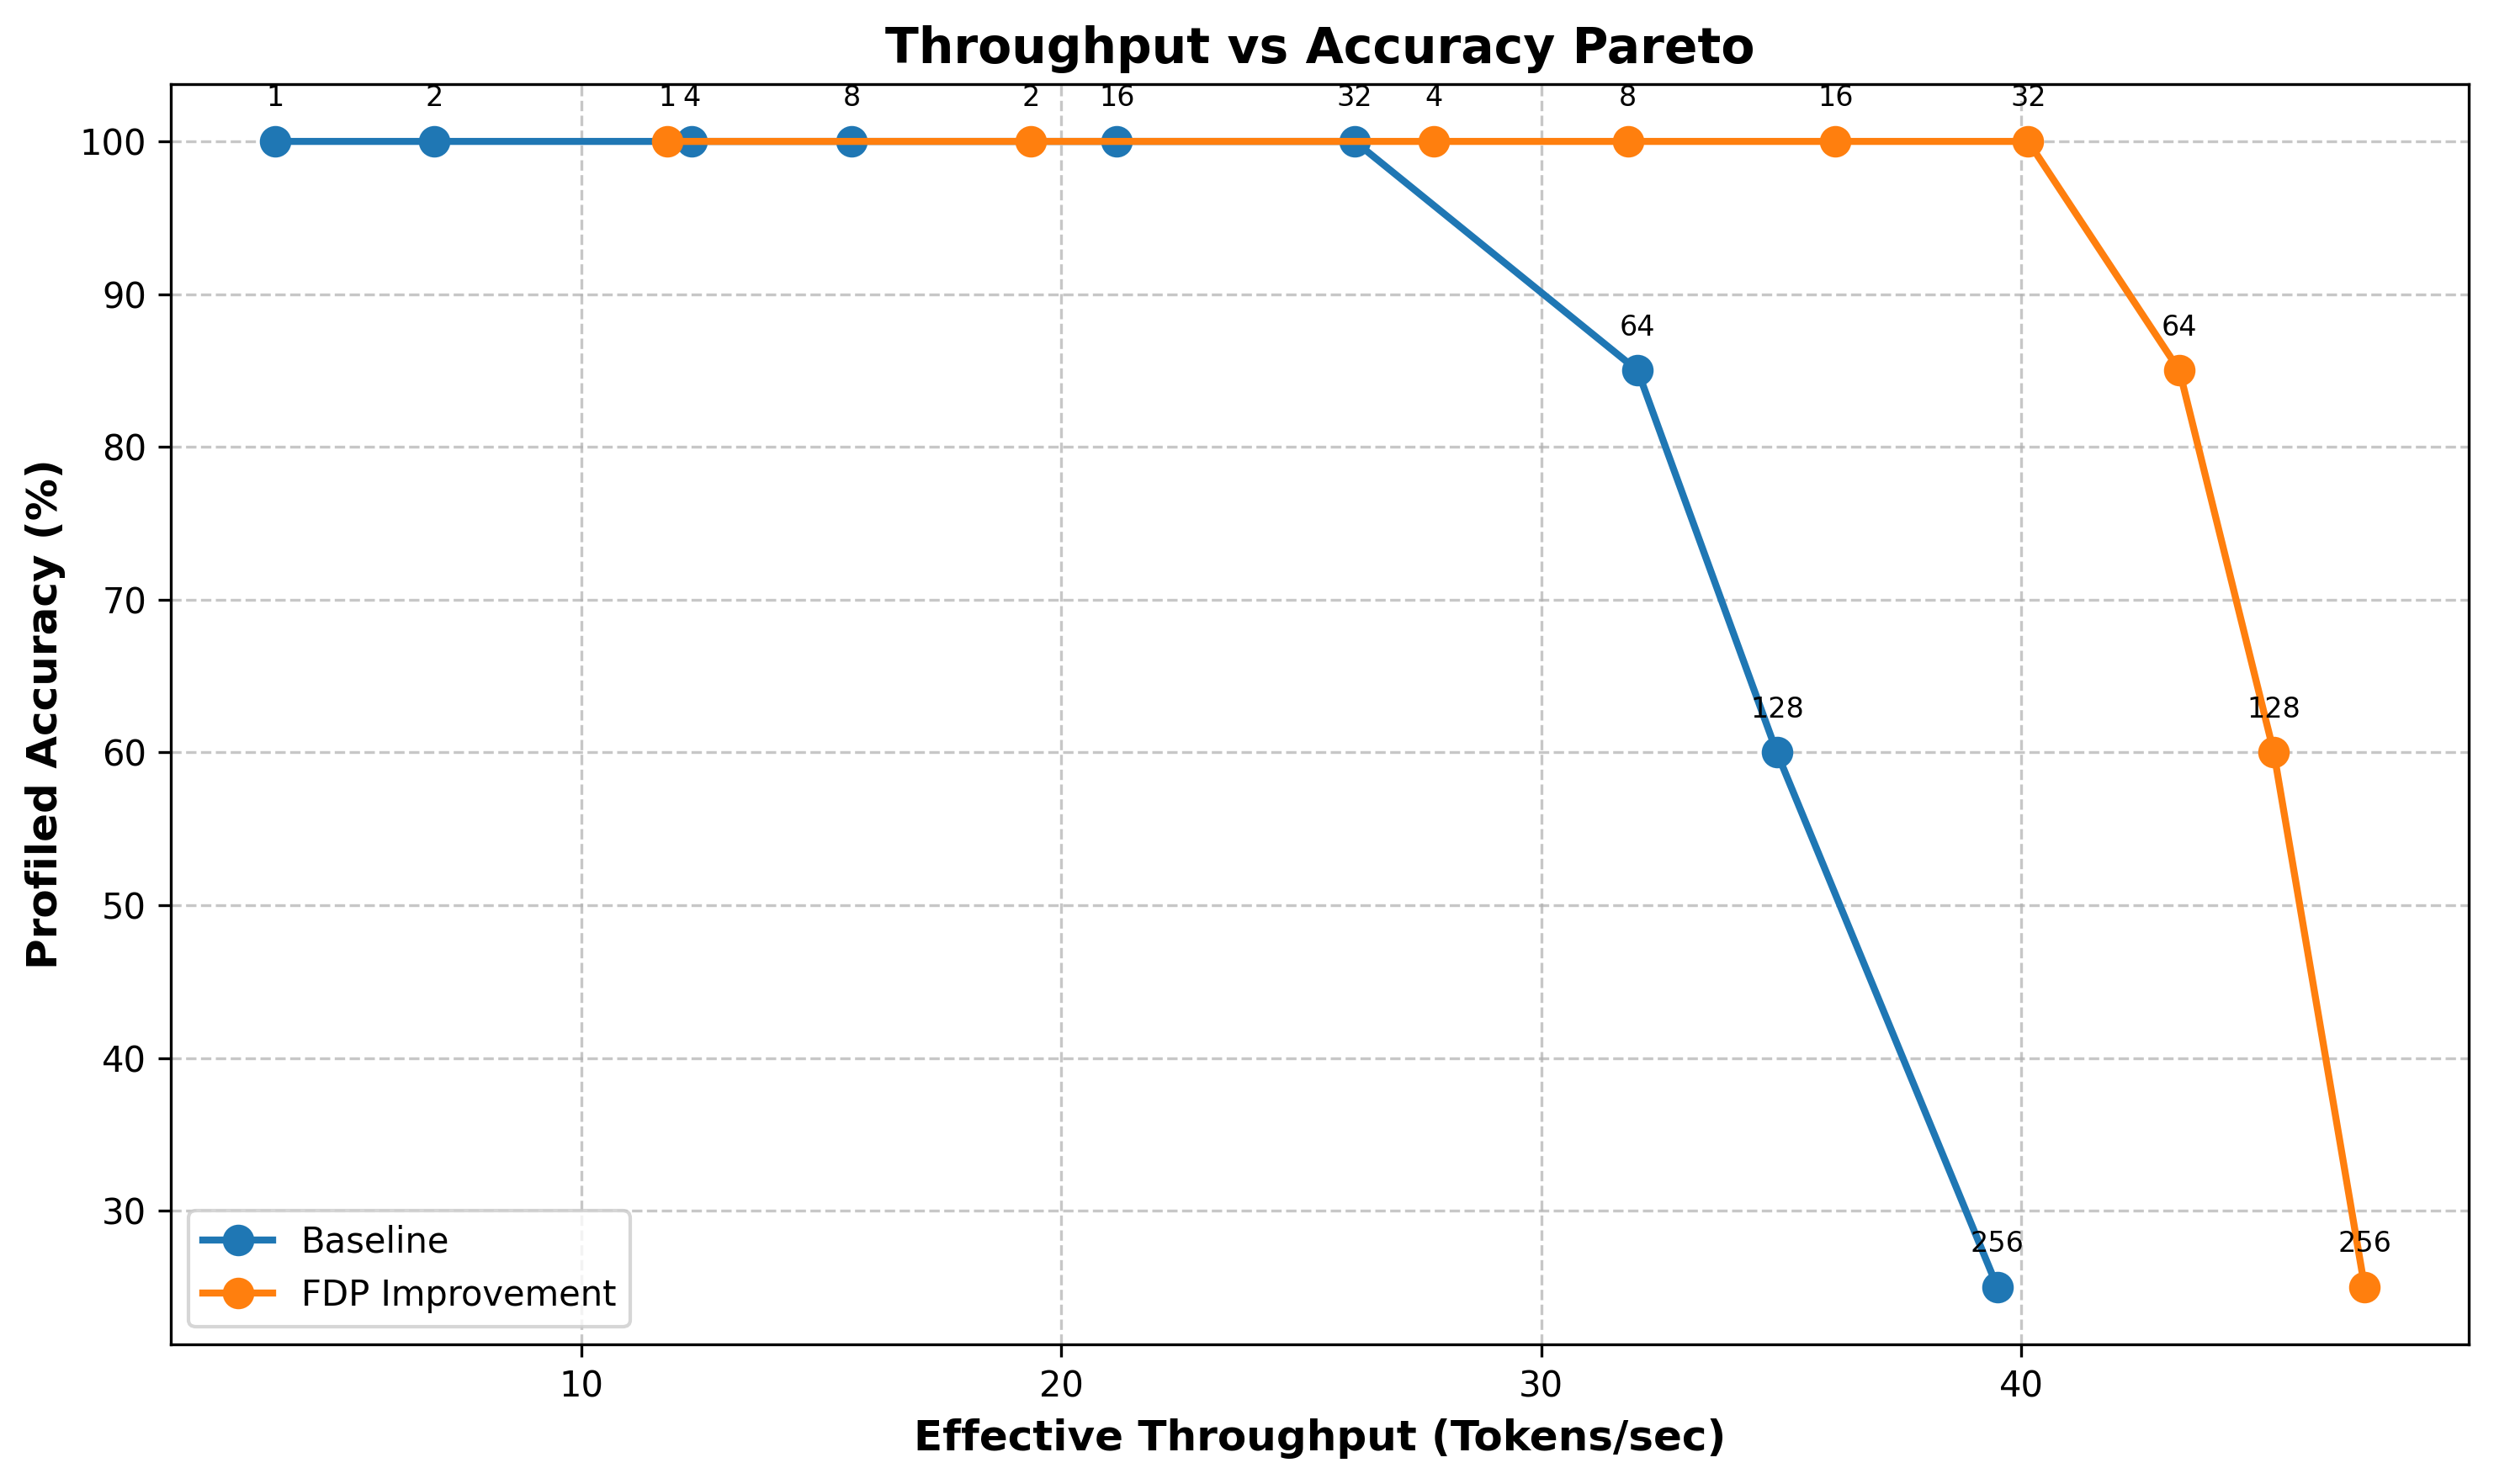
\includegraphics[width=\textwidth]{../outputs/phase3/fdp_results/Meta-Llama-3.1-8B-4bit/pareto_combined.png}
                \caption{Llama-3.1-8B}
                \label{fig:pareto_fdp_llama31}
            \end{subfigure}
            \hfill
            \begin{subfigure}[c]{0.32\textwidth}
                \centering
                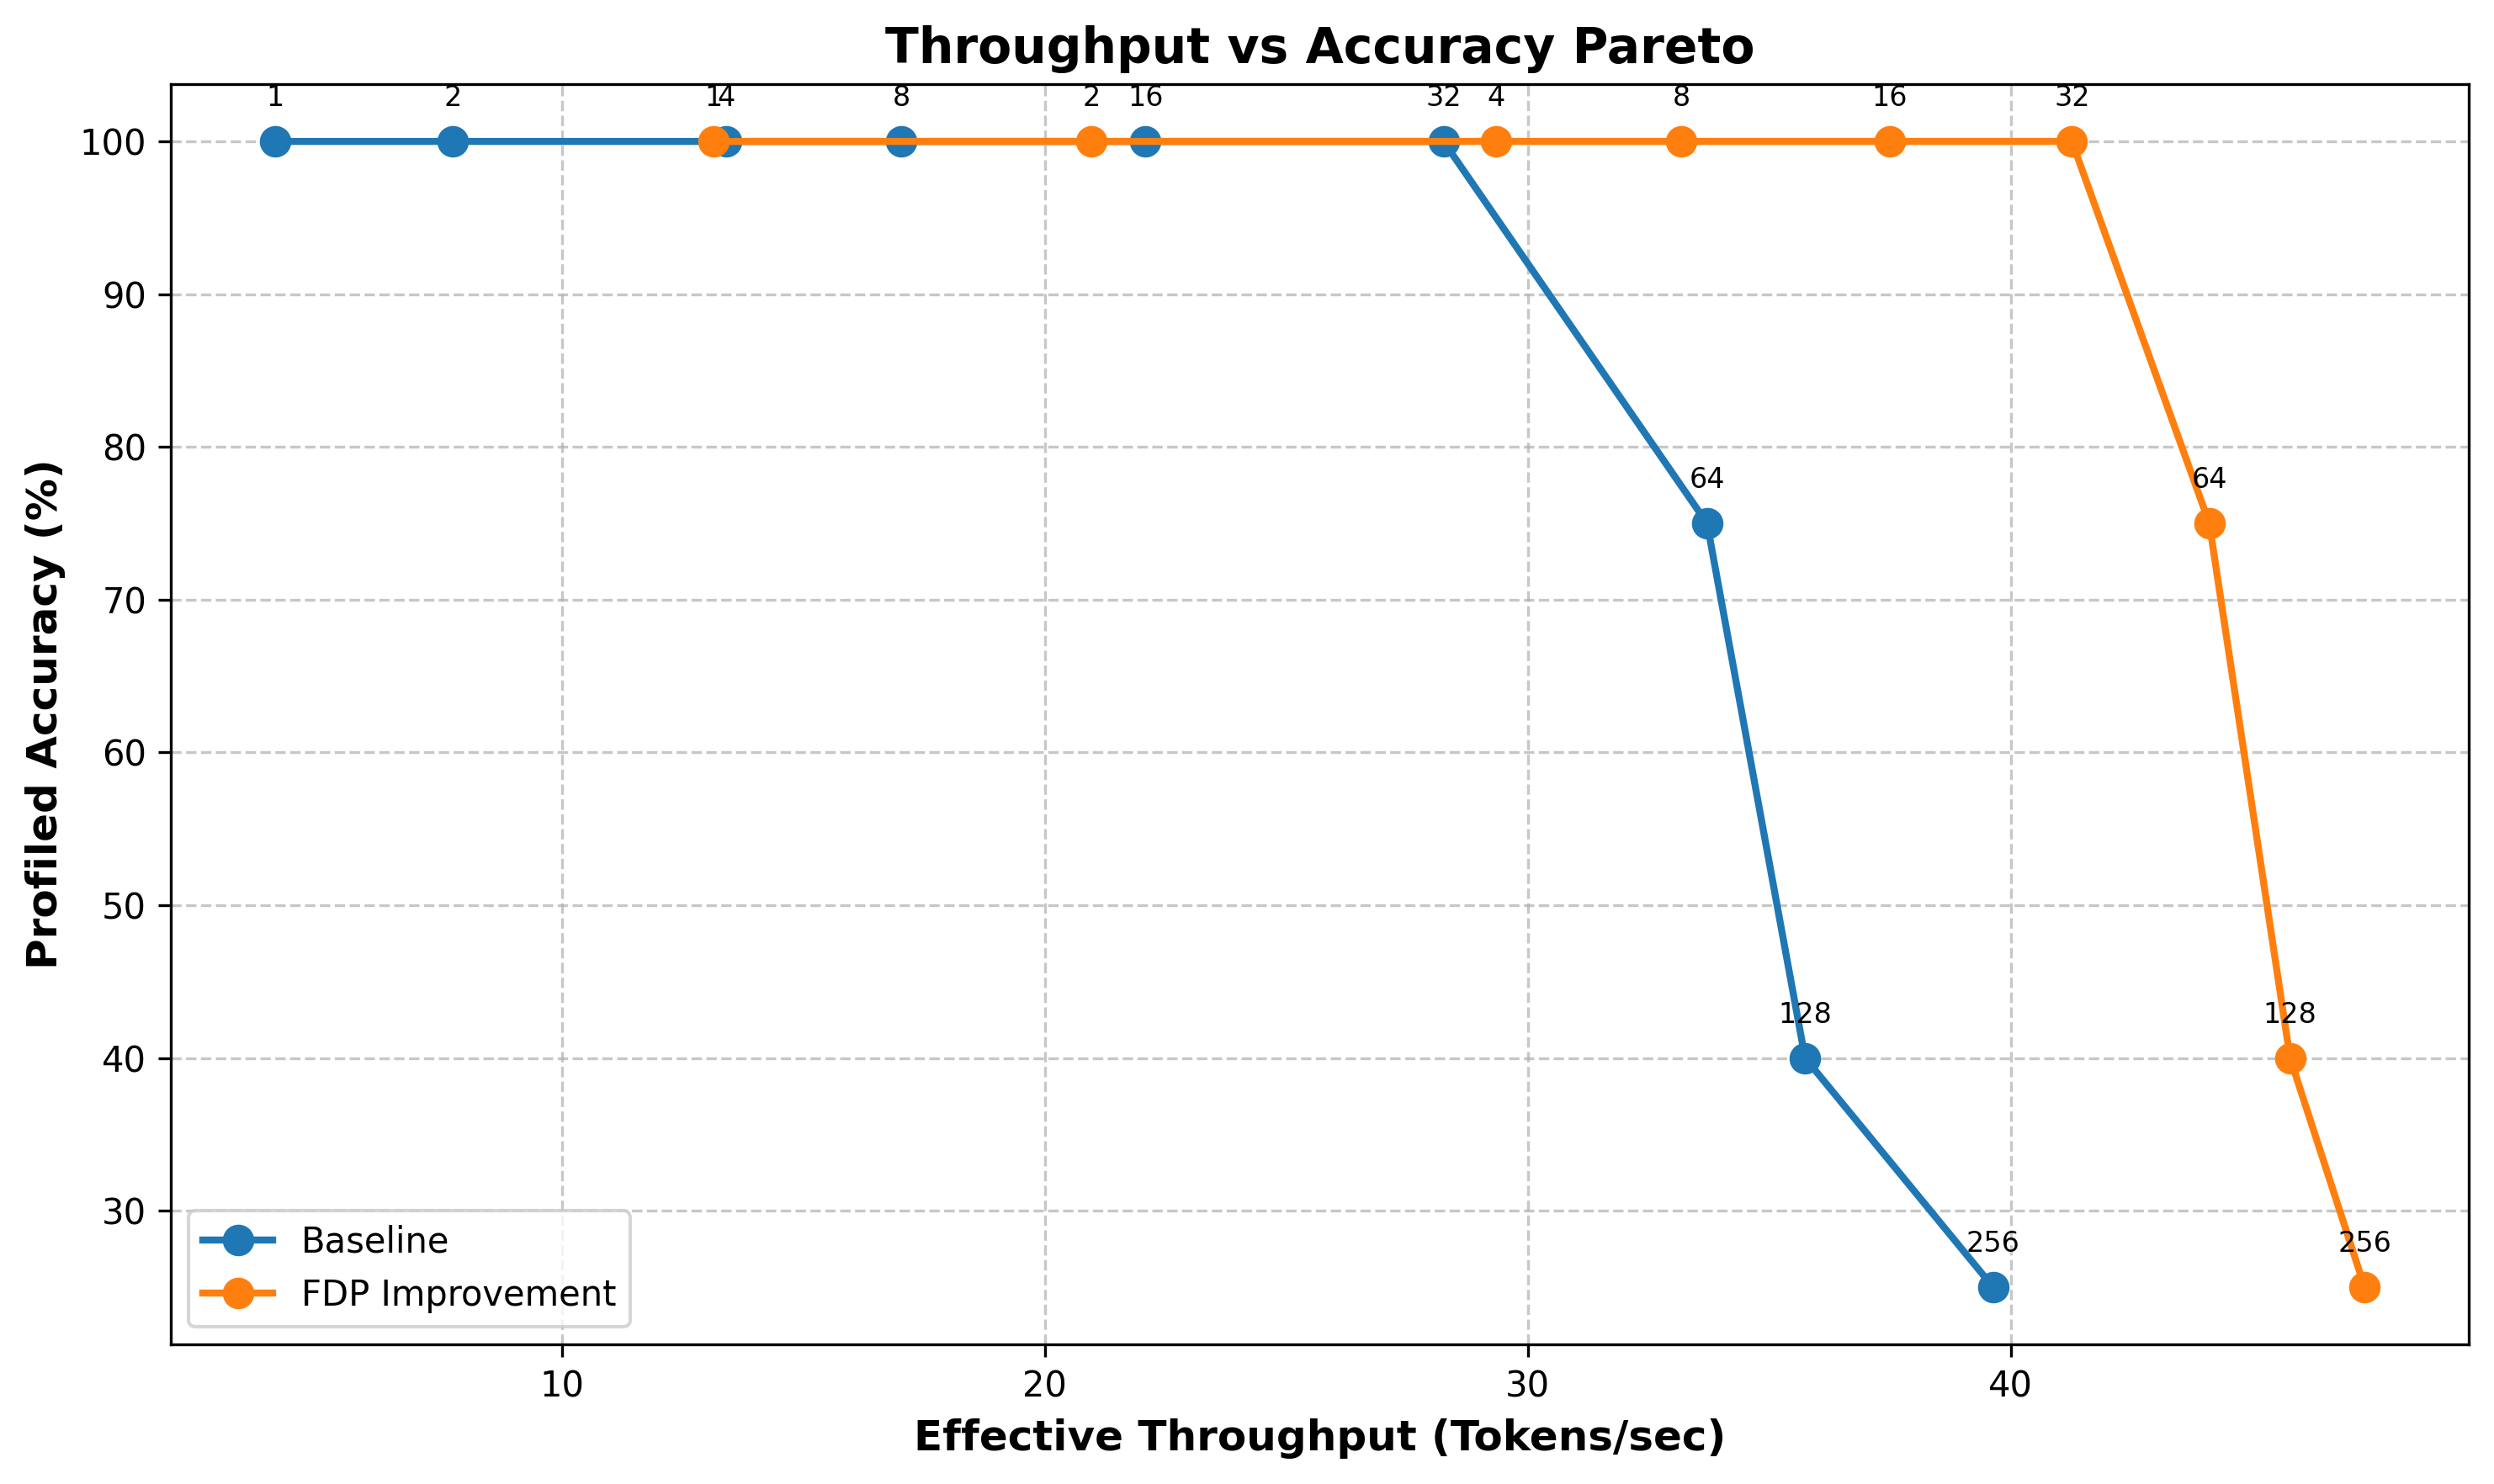
\includegraphics[width=\textwidth]{../outputs/phase3/fdp_results/Meta-Llama-3.2-3B-8bit/pareto_combined.png}
                \caption{Llama-3.2-3B}
                \label{fig:pareto_fdp_llama32}
            \end{subfigure}
            \hfill
            \begin{subfigure}[c]{0.32\textwidth}
                \centering
                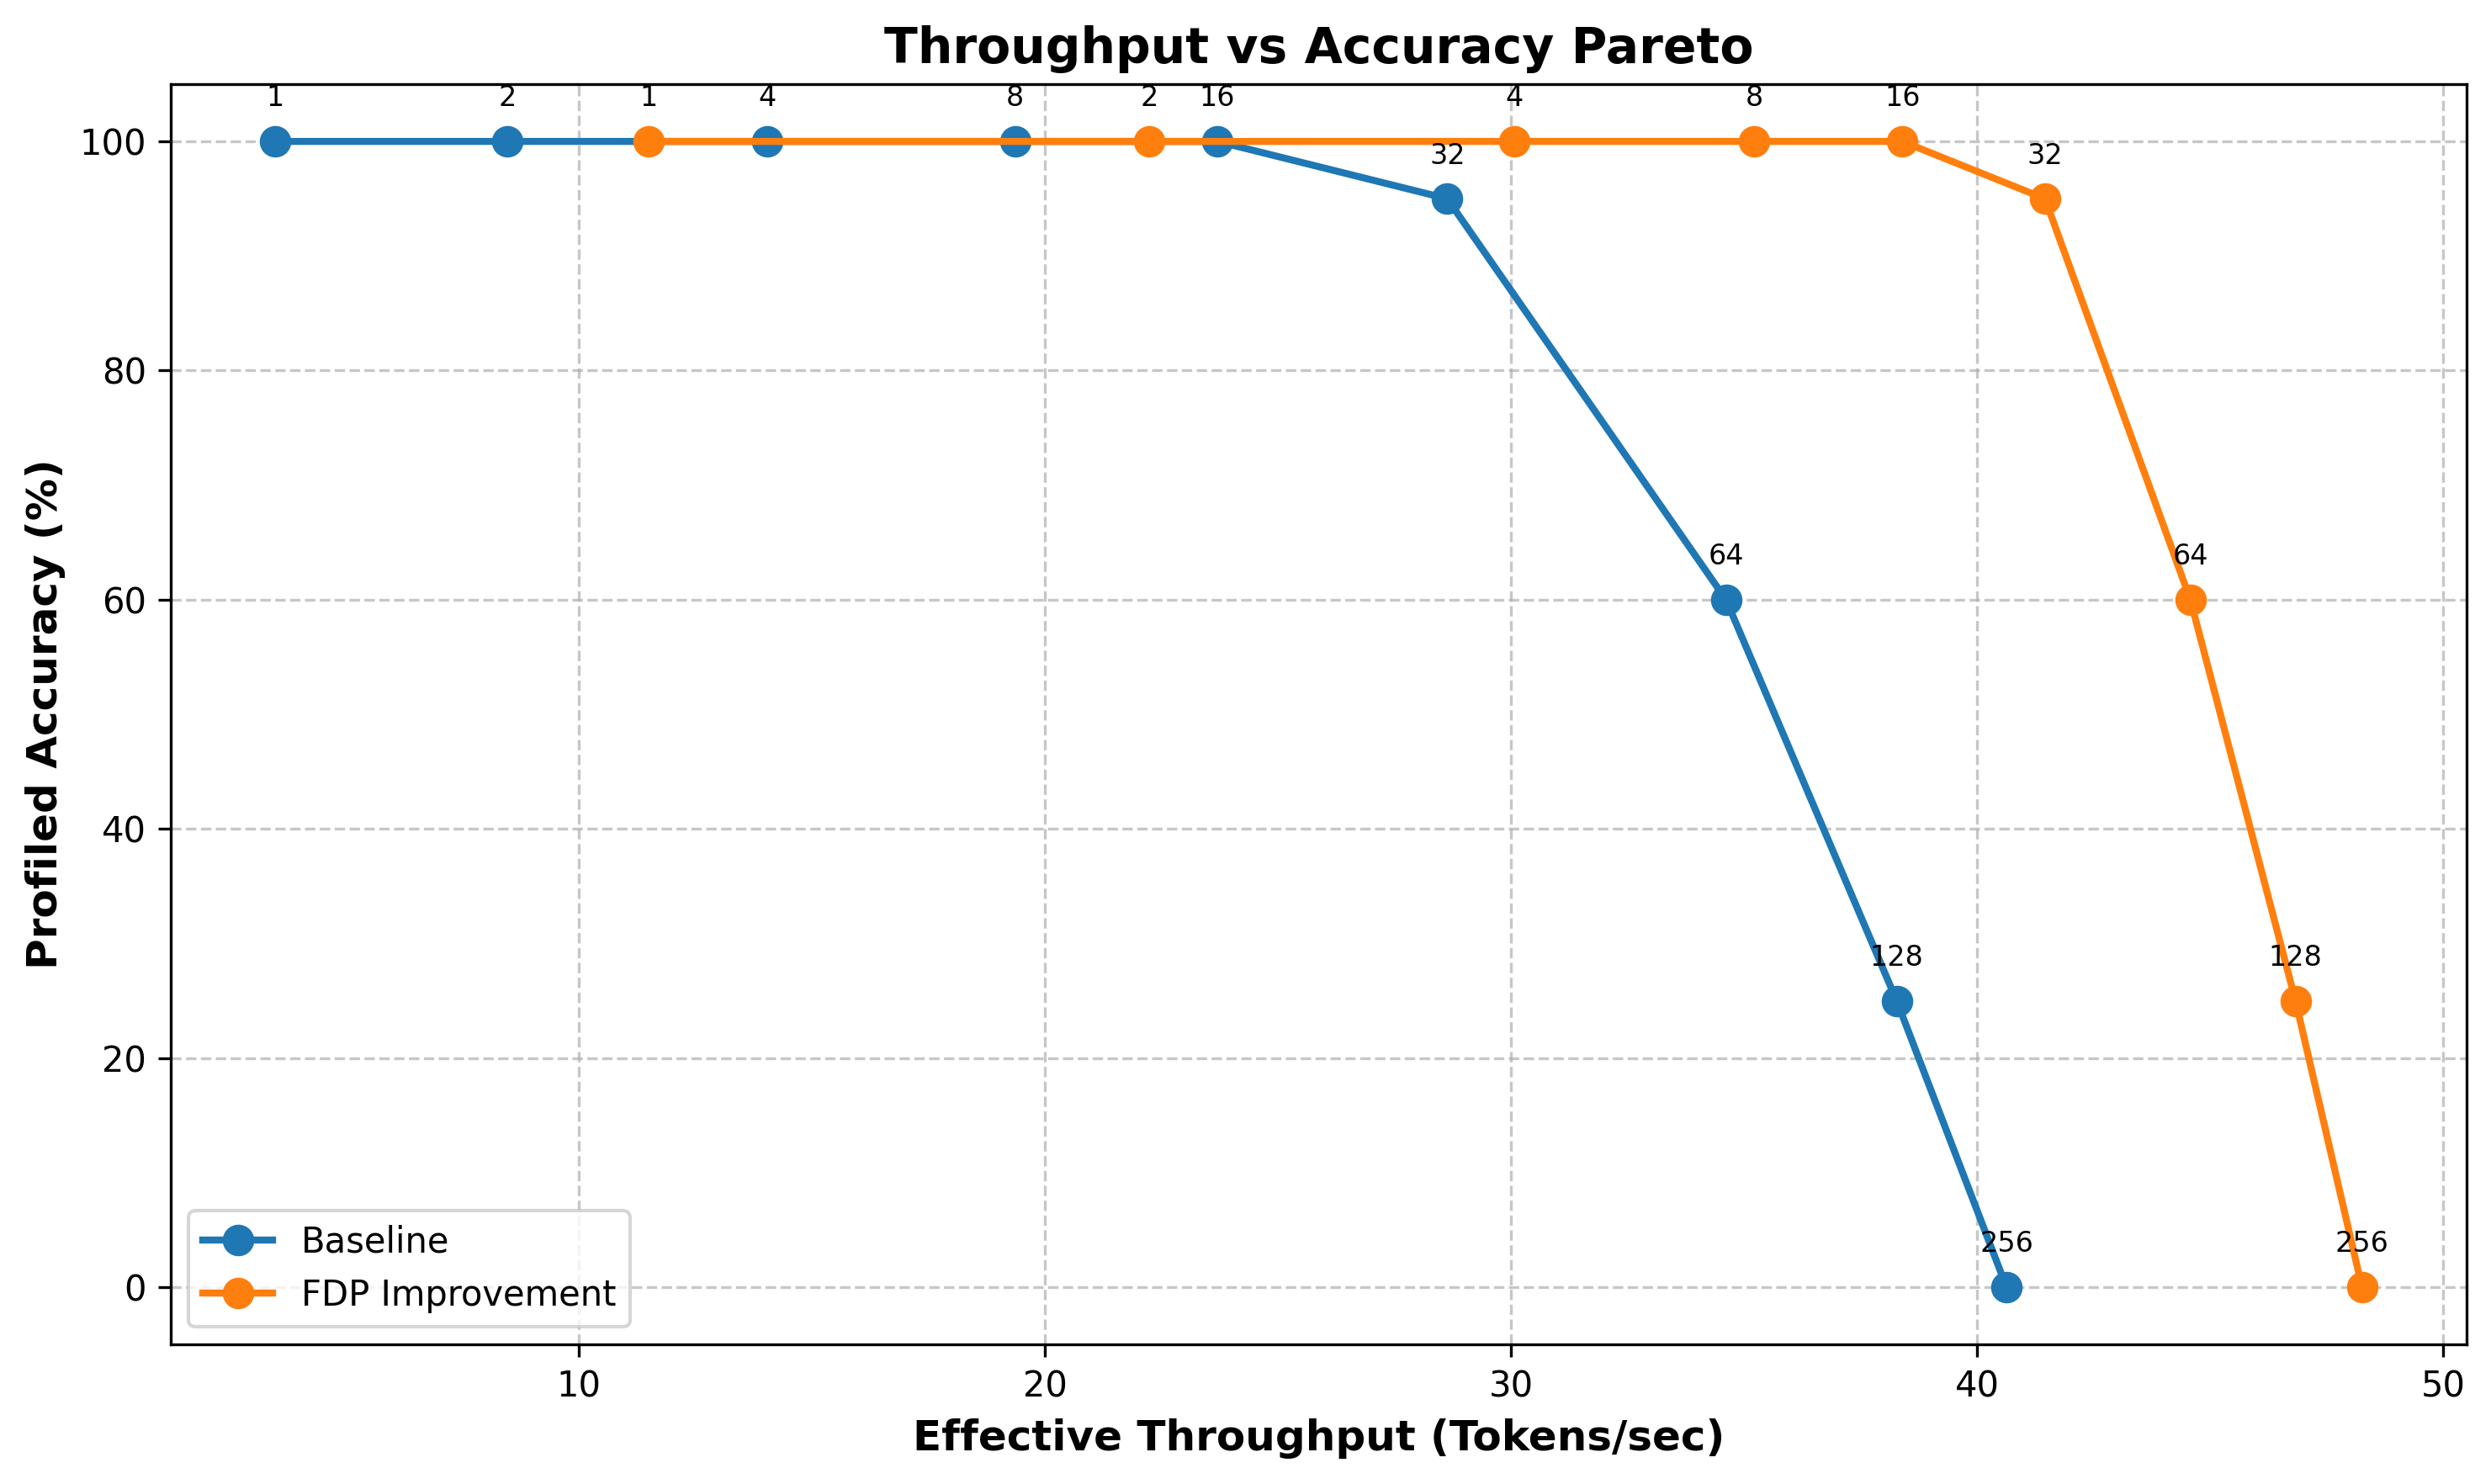
\includegraphics[width=\textwidth]{../outputs/phase3/fdp_results/Qwen2.5-7B-4bit/pareto_combined.png}
                \caption{Qwen-2.5-7B}
                \label{fig:pareto_fdp_qwen}
            \end{subfigure}
            \caption{Pareto Frontiers under FDP across three LLMs. The zero-GC penalty and data striping push the frontiers significantly outward, enabling high throughput even at smaller, more accurate block sizes.}
            \label{fig:pareto_fdp_combined}
        \end{figure*}
        
        These results demonstrate that under the assumed FDP benefits, it allows the use of much smaller block sizes (e.g. 4 tokens) while maintaining the same level of performance. The ability to operate at such small block sizes may be beneficial for less accurate models, or perhaps for different tasks, that performs better and finer granularity.

\section{Conclusion \& Limitations}
    In this project, I evaluated the \textit{SolidAttention}\cite{solidattention} framework on memory-constrained PCs, focusing on the tension between KV cache block size (which controls SSD I/O efficiency) and LLM generative accuracy (which requires precise token retrieval).
    
    Using a simulated implementation of \textit{SolidAttention}, I began by confirming the general trends presented in the original paper, specifically the accuracy drop-off as block size increases, and the general shape of the Pareto frontier. My results across all three tested models generally aligned with the original paper's findings, and further analyses on miss rate showed that the system's performance is asymmetric with respect to miss rate variations. 
    
    Next, I suggested and simulated the potential use of NVMe Flexible Data Placement (FDP). While offloading to an SSD is an effective strategy to avoid hardware memory limits, under the assumptions of the simulator, eliminating GC-related stalls and improving effective SSD bandwidth substantially increases the achievable throughput.

    Under the assumed bandwidth improvement, these results yield several architectural conclusions:
    \begin{enumerate}
        \item The baseline configuration is sufficiently I/O-sensitive that increasing effective SSD bandwidth substantially improves inference throughput.
        \item By utilizing FDP to stripe blocks across multiple parallel flash channels, it effectively multiplies the available read bandwidth. This allows the system to better mask SSD latency behind the GPU's computation window, moving the inference pipeline from an I/O-bound state to a compute-bound state.
        \item The rightward shift of the Pareto fronts suggests that algorithmic innovations, such as those presented by \textit{SolidAttention}\cite{solidattention}, must be co-designed with physical storage layout in mind, to maximize generative inference performance on memory-constrained edge devices.
    \end{enumerate}

    This project relied on several assumptions that should be noted as limitations:
    \begin{itemize}
        \item The FDP results are simulation-based, not measurements on an FDP-enabled SSD.
        \item The simulator does not explicitly model SSD behavior or computation/I/O overlap.
        \item The NIAH experiment measures retrieval accuracy, and does not reproduce SolidAttention's LongBench recall\slash accuracy evaluation.
    \end{itemize}

    Future work could include implementing FDP directly in inference frameworks, such as \texttt{llama.cpp}, and test these latency gains on physical FDP-compliant drives.

\begin{thebibliography}{00}
    \bibitem{solidattention}
        X. Zheng, D. Wei, J. Gao, Y. Song, Z. Mi, and H. Chen, ``SolidAttention: Low-Latency SSD-based Serving on Memory-Constrained PCs,'' in \textit{Proceedings of the 24th USENIX Conference on File and Storage Technologies (FAST '26)}, 2026.

    \bibitem{fdp_overview}
        Samsung Semiconductor, ``NVMe FDP: A Promising New SSD Data Placement Approach,'' \url{semiconductor.samsung.com/news-events/tech-blog/nvme-fdp-a-promising-new-ssd-data-placement-approach/}.
\end{thebibliography}

\end{document}
